\documentclass[fleqn,10pt]{wlscirep}
\usepackage[utf8]{inputenc}
\usepackage[T1]{fontenc}
\usepackage{makecell}

\title{Supplementary Information}


\author[1,2,*,\textsuperscript{\textdagger}]{Carmen Cabrera}
\author[1]{Miguel González-Leonardo}
\author[1,3]{Andrea Nasuto}
\author[2]{Ruth Neville}
\author[1,\textsuperscript{\textdagger}]{Francisco Rowe}
\affil[1]{Geographic Data Science Lab, Department of Geography and Planning, University of Liverpool, Liverpool, UK}
\affil[2]{Centre for Advanced Spatial Analysis, University College London, London, UK}
\affil[3]{Institute for Quantitative Social Science, Harvard University, Cambridge, US}


\affil[*]{Corresponding author: c.cabrera@liverpool.ac.uk}

\affil[ \textsuperscript{\textdagger}]{These authors have contributed equally to this study.}


%\keywords{Keyword1, Keyword2, Keyword3}


\begin{abstract}
Urban mobility is central to economic activity, social inclusion and access to services. COVID-19 caused disruptions to mobility globally, yet its long-term impacts in less developed countries remain poorly understood. Using an unprecedentedly large dataset of $>$170 million mobile phone records from Meta-Facebook users in Argentina, Chile and Colombia (April 2020–May 2022), we find sustained changes in mobility across socioeconomic and rural–urban gradients. We reveal that mobility recorded the sharpest declines and remained below pre-pandemic levels in most high-density and most affluent areas, while low-density and more deprived communities returned to baseline. These differences reflect the scale of the initial mobility shock, rather than subsequent recovery rates. Our findings reveal how a global shock can entrench disparities in human mobility, with implications for economic resilience, social inclusion and urban planning in unequal nations. Our study underscores the need for proactive policies to prevent long‑lasting inequalities in mobility
\end{abstract}

\begin{document}

\flushbottom

\maketitle
% * <john.hammersley@gmail.com> 2015-02-09T12:07:31.197Z:
%
%  Click the title above to edit the author information and abstract
%

% * <john.hammersley@gmail.com> 2015-02-09T12:07:31.197Z:
%
%  Click the title above to edit the author information and abstract

\section{Processing Facebook data}

\subsection{Missing values}

\begin{table}[h!]
\centering
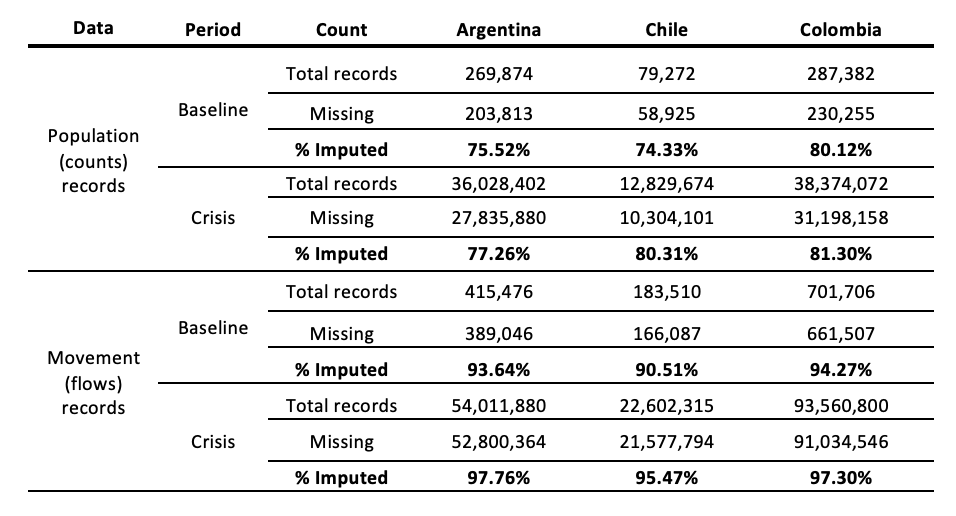
\includegraphics[width=0.9\linewidth]{supplementary/missing/SF-missing-data-table-r1.png}
\caption{Summary of missing and imputed values in the Facebook Population and Facebook Movements datasets during the baseline and crisis periods for Argentina, Chile and Colombia. The table reports total records, number of missing observations and the percentage of data imputed.}
\end{table}

\newpage

\begin{figure}[h!]
\centering
\includegraphics[width=.7\linewidth]{supplementary/missing/SF-missing.png}
\caption{Facebook Population baseline records corresponding to Monday, for Argentina, Chile and Colombia. The first row shows the original records, which include a high proportion of missing values. The second row shows the imputed baseline following a regression model with Worldpop data. This figure provides descriptive insight into the baseline population measure used in the analysis.}
\label{missing-baseline}
\end{figure}

\newpage

\subsection{Relationship between WorldPop population and Facebook Population baseline data for each day of the week}

\begin{figure}[h!]
\centering
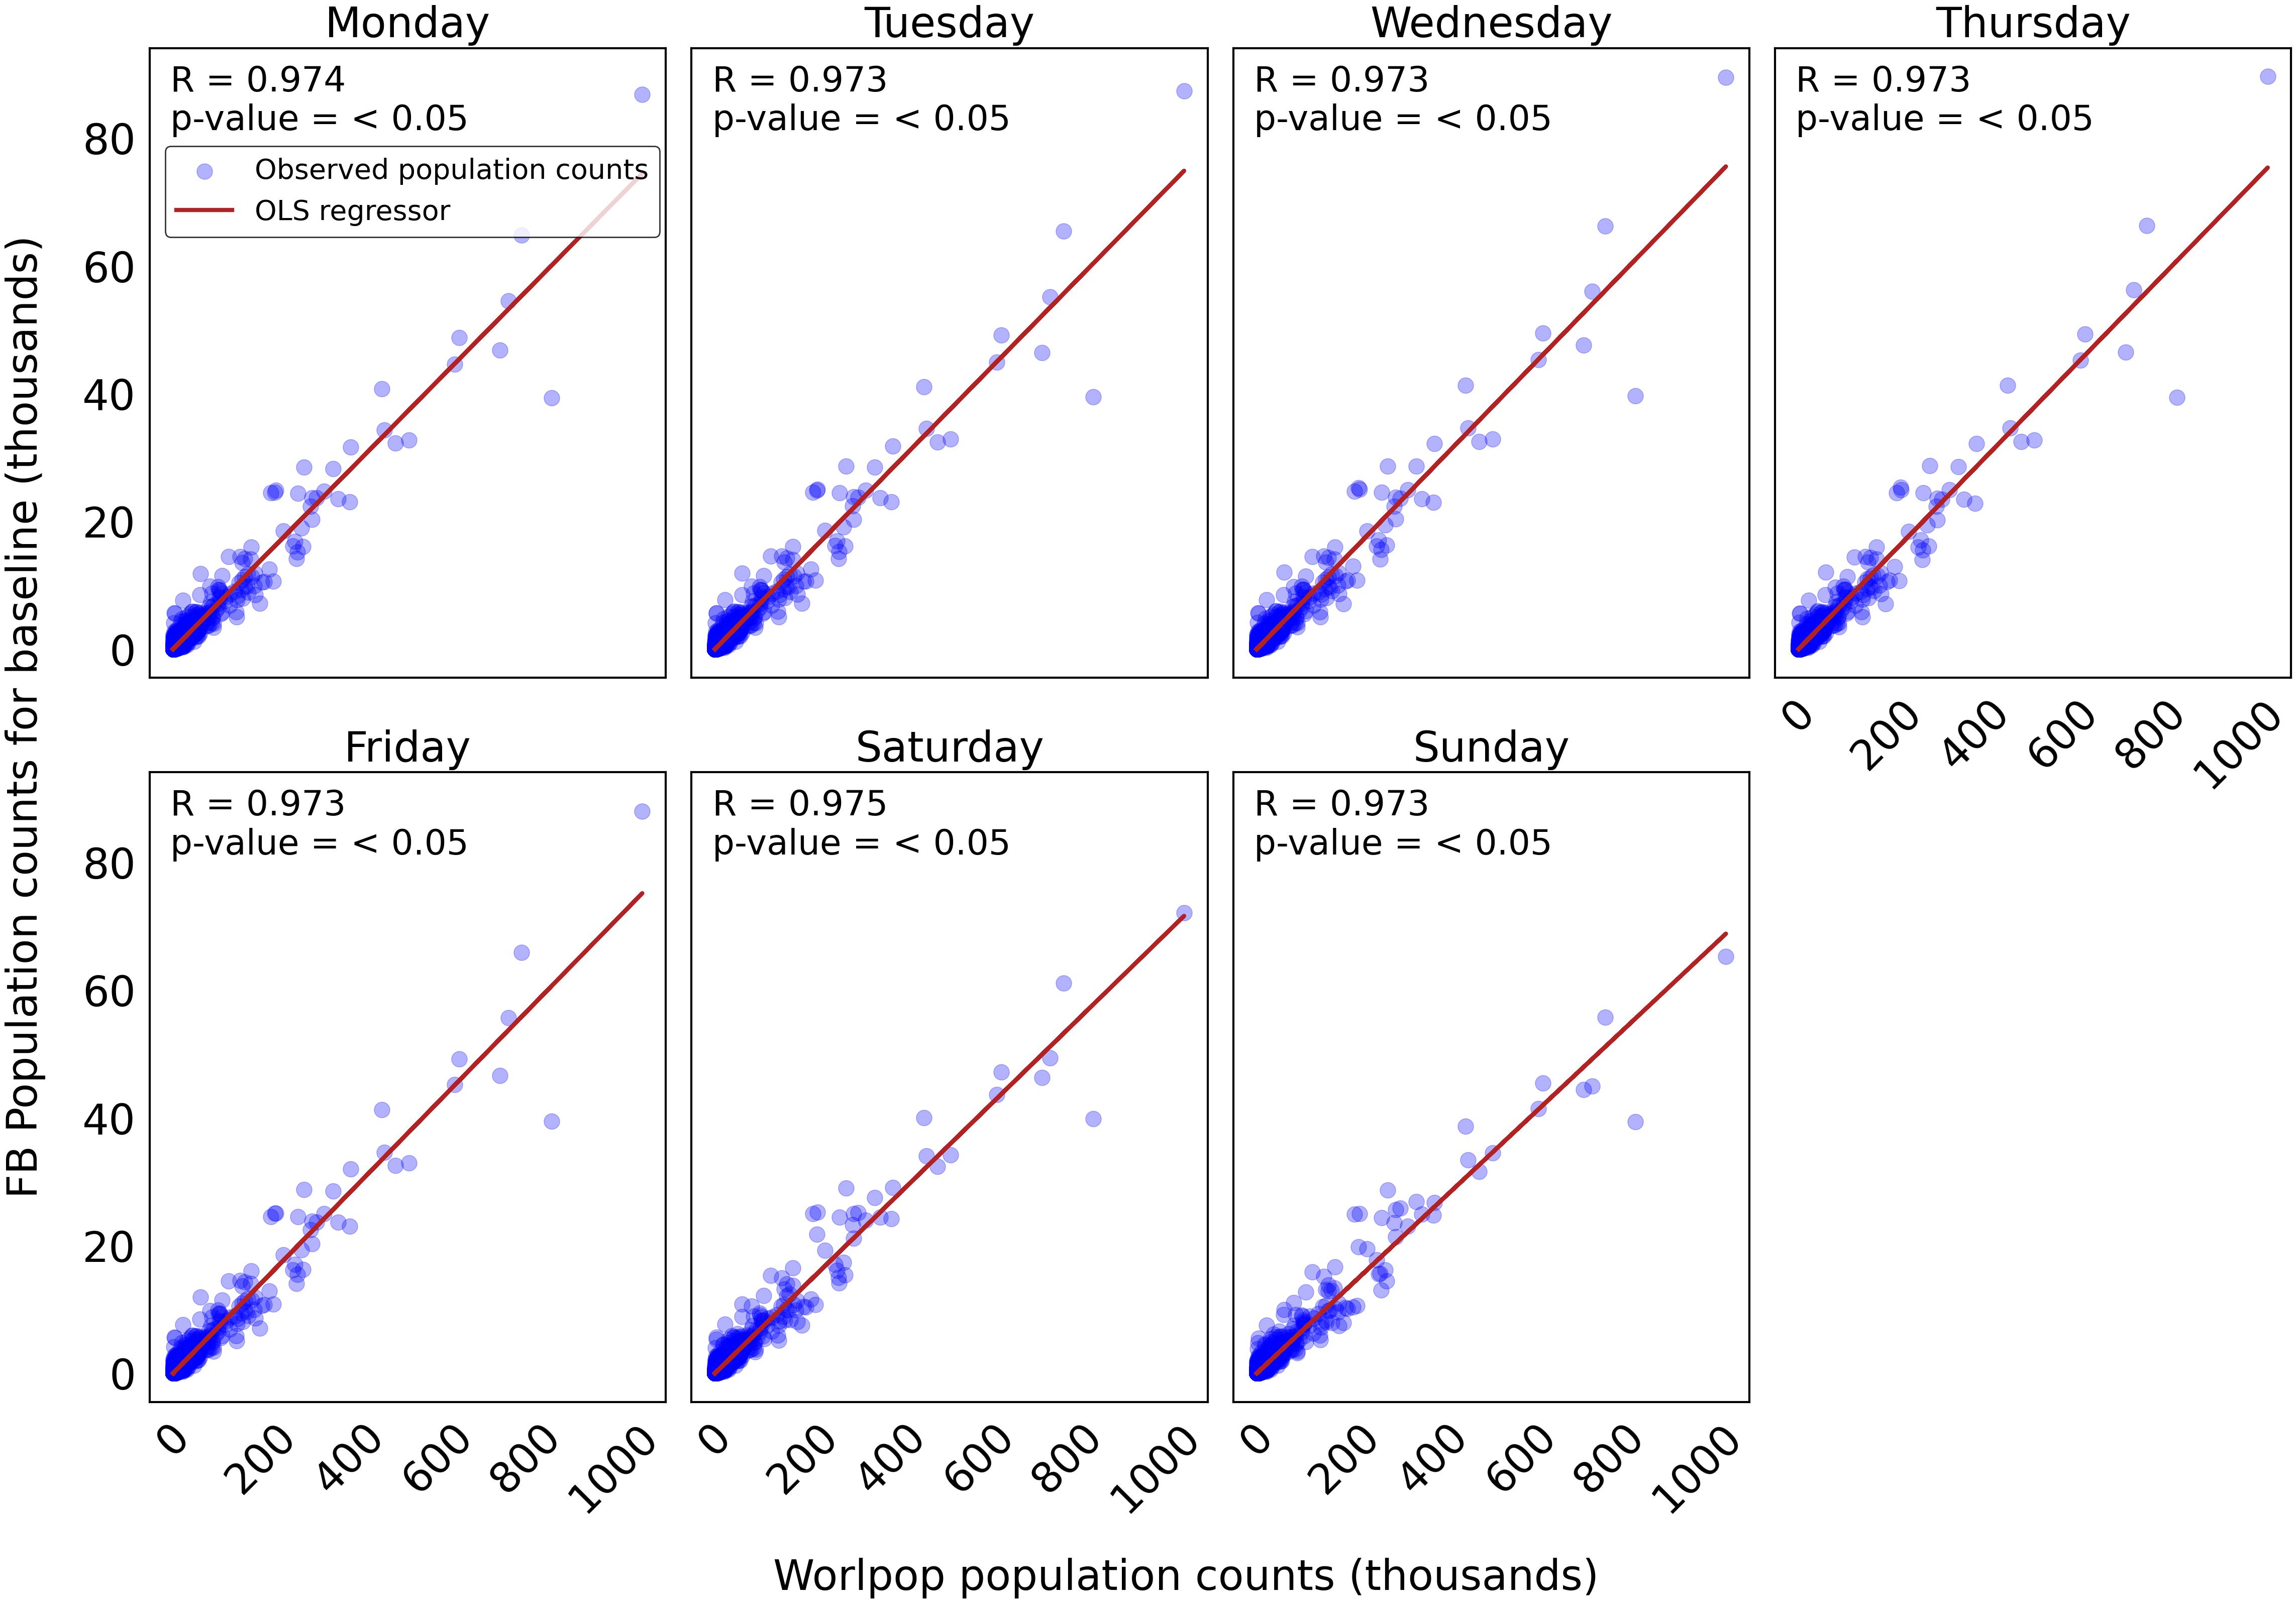
\includegraphics[width=\linewidth]{supplementary/correlation/correlation-wp-fb-pop-baseline-ARG.png}
\caption{Correlation between Worldpop population counts and Facebook Population counts during the baseline period in Argentina, for each day of the week.}
\label{correlation-wp-fbpop-ARG}
\end{figure}

\newpage

\begin{figure}[h!]
\centering
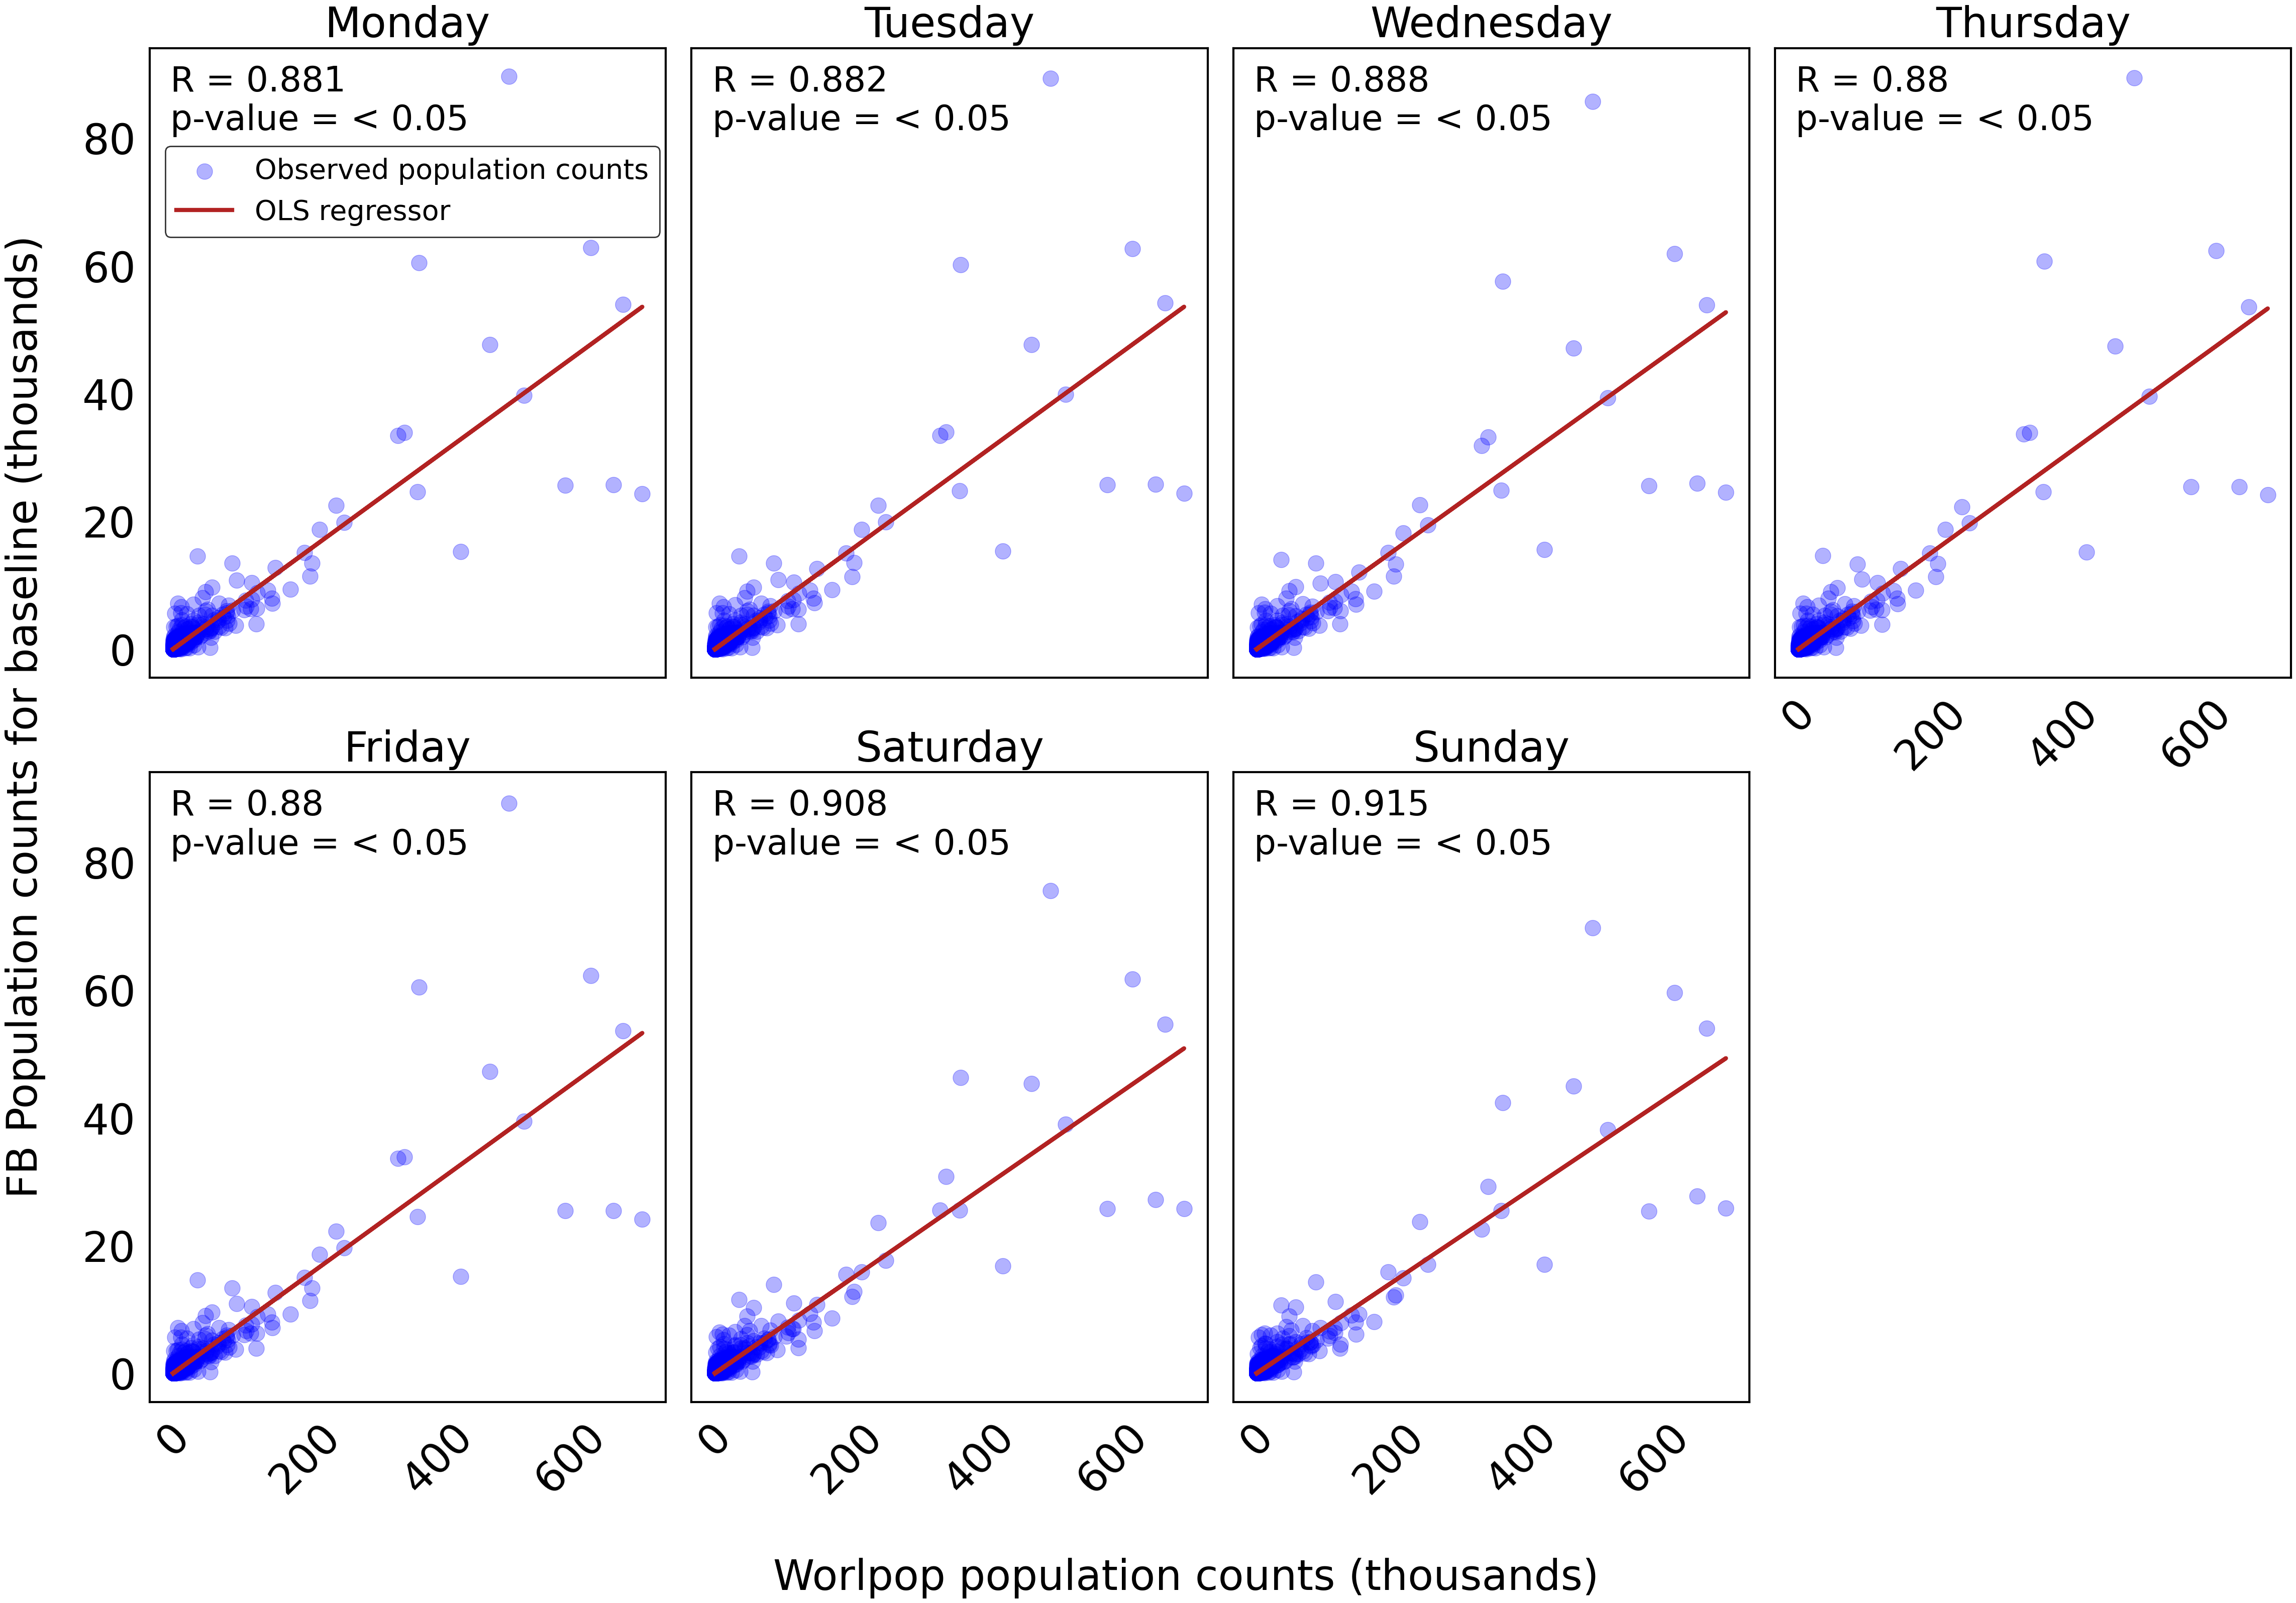
\includegraphics[width=\linewidth]{supplementary/correlation/correlation-wp-fb-pop-baseline-CHL.png}
\caption{Correlation between Worldpop population counts and Facebook Population counts during the baseline period in Chile, for each day of the week.}
\label{correlation-wp-fbpop-CHL}
\end{figure}

\newpage

\begin{figure}[h!]
\centering
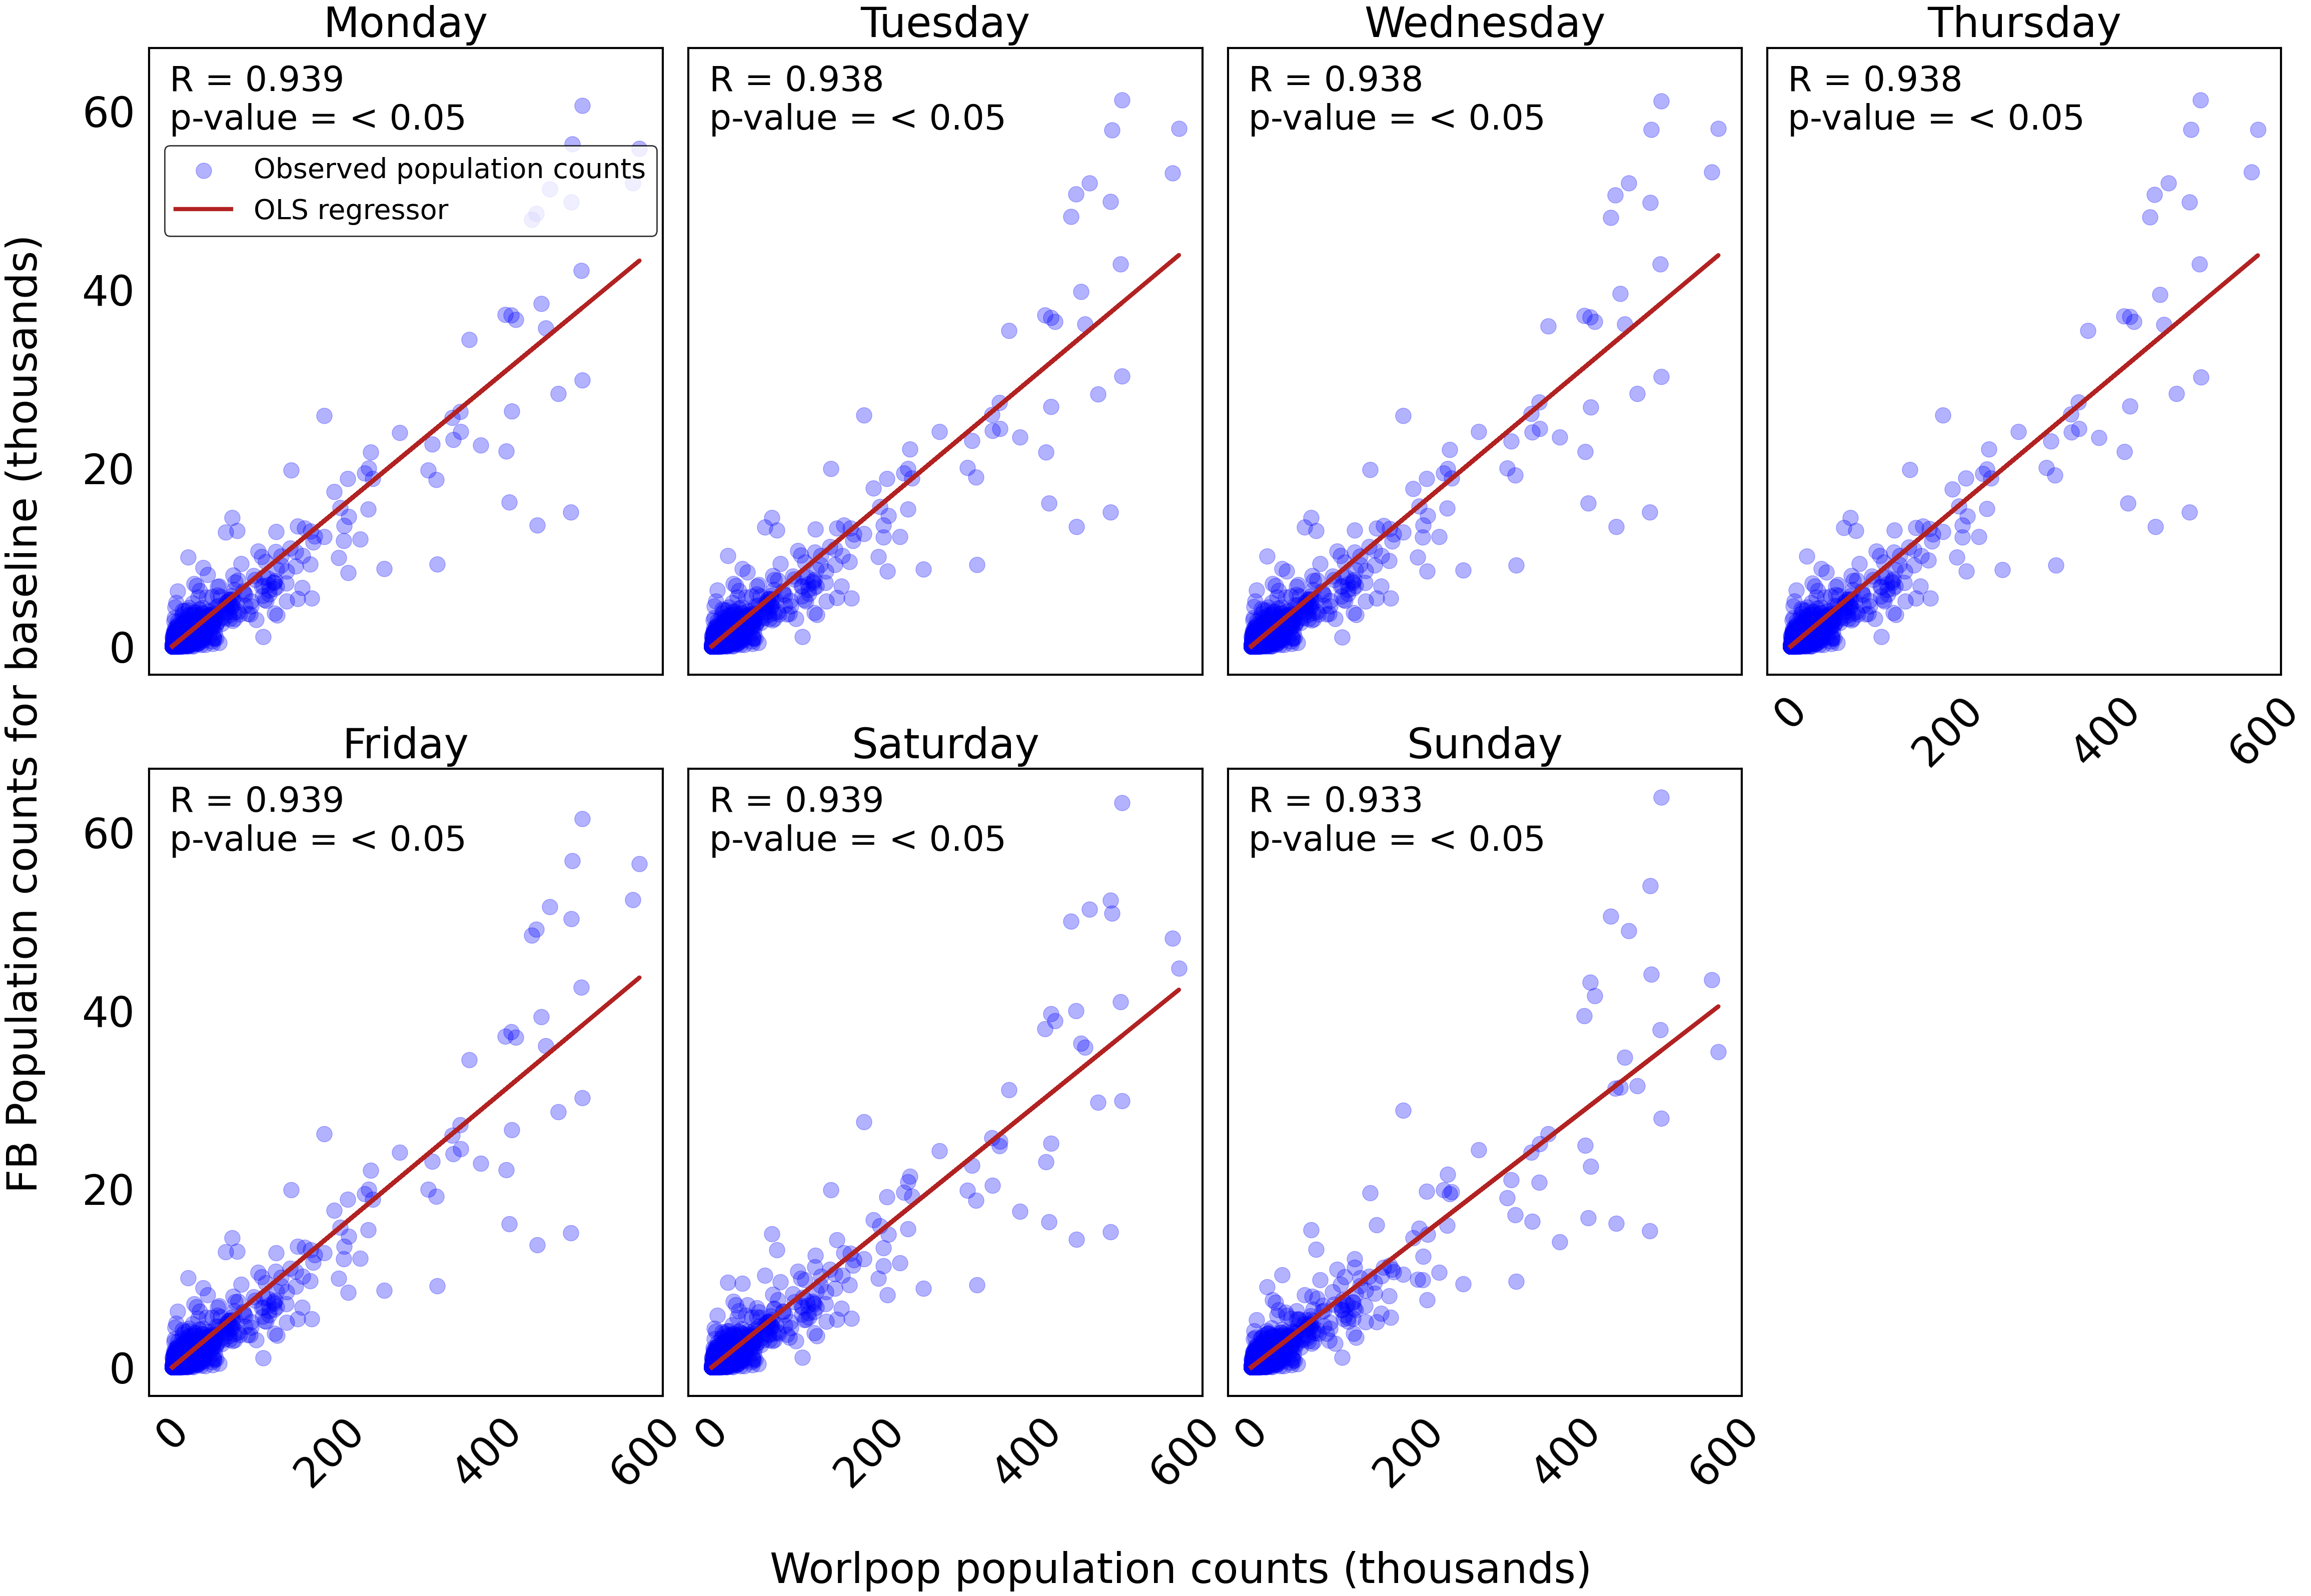
\includegraphics[width=\linewidth]{supplementary/correlation/correlation-wp-fb-pop-baseline-COL.png}
\caption{Correlation between Worldpop population counts and Facebook Population counts during the baseline period in Colombia, for each day of the week.}
\label{correlation-wp-fbpop-COL}
\end{figure}

\newpage

\subsection{Assessing results of spatial interaction model for imputing missing number of movements in baseline}

\begin{figure}[h!]
\centering
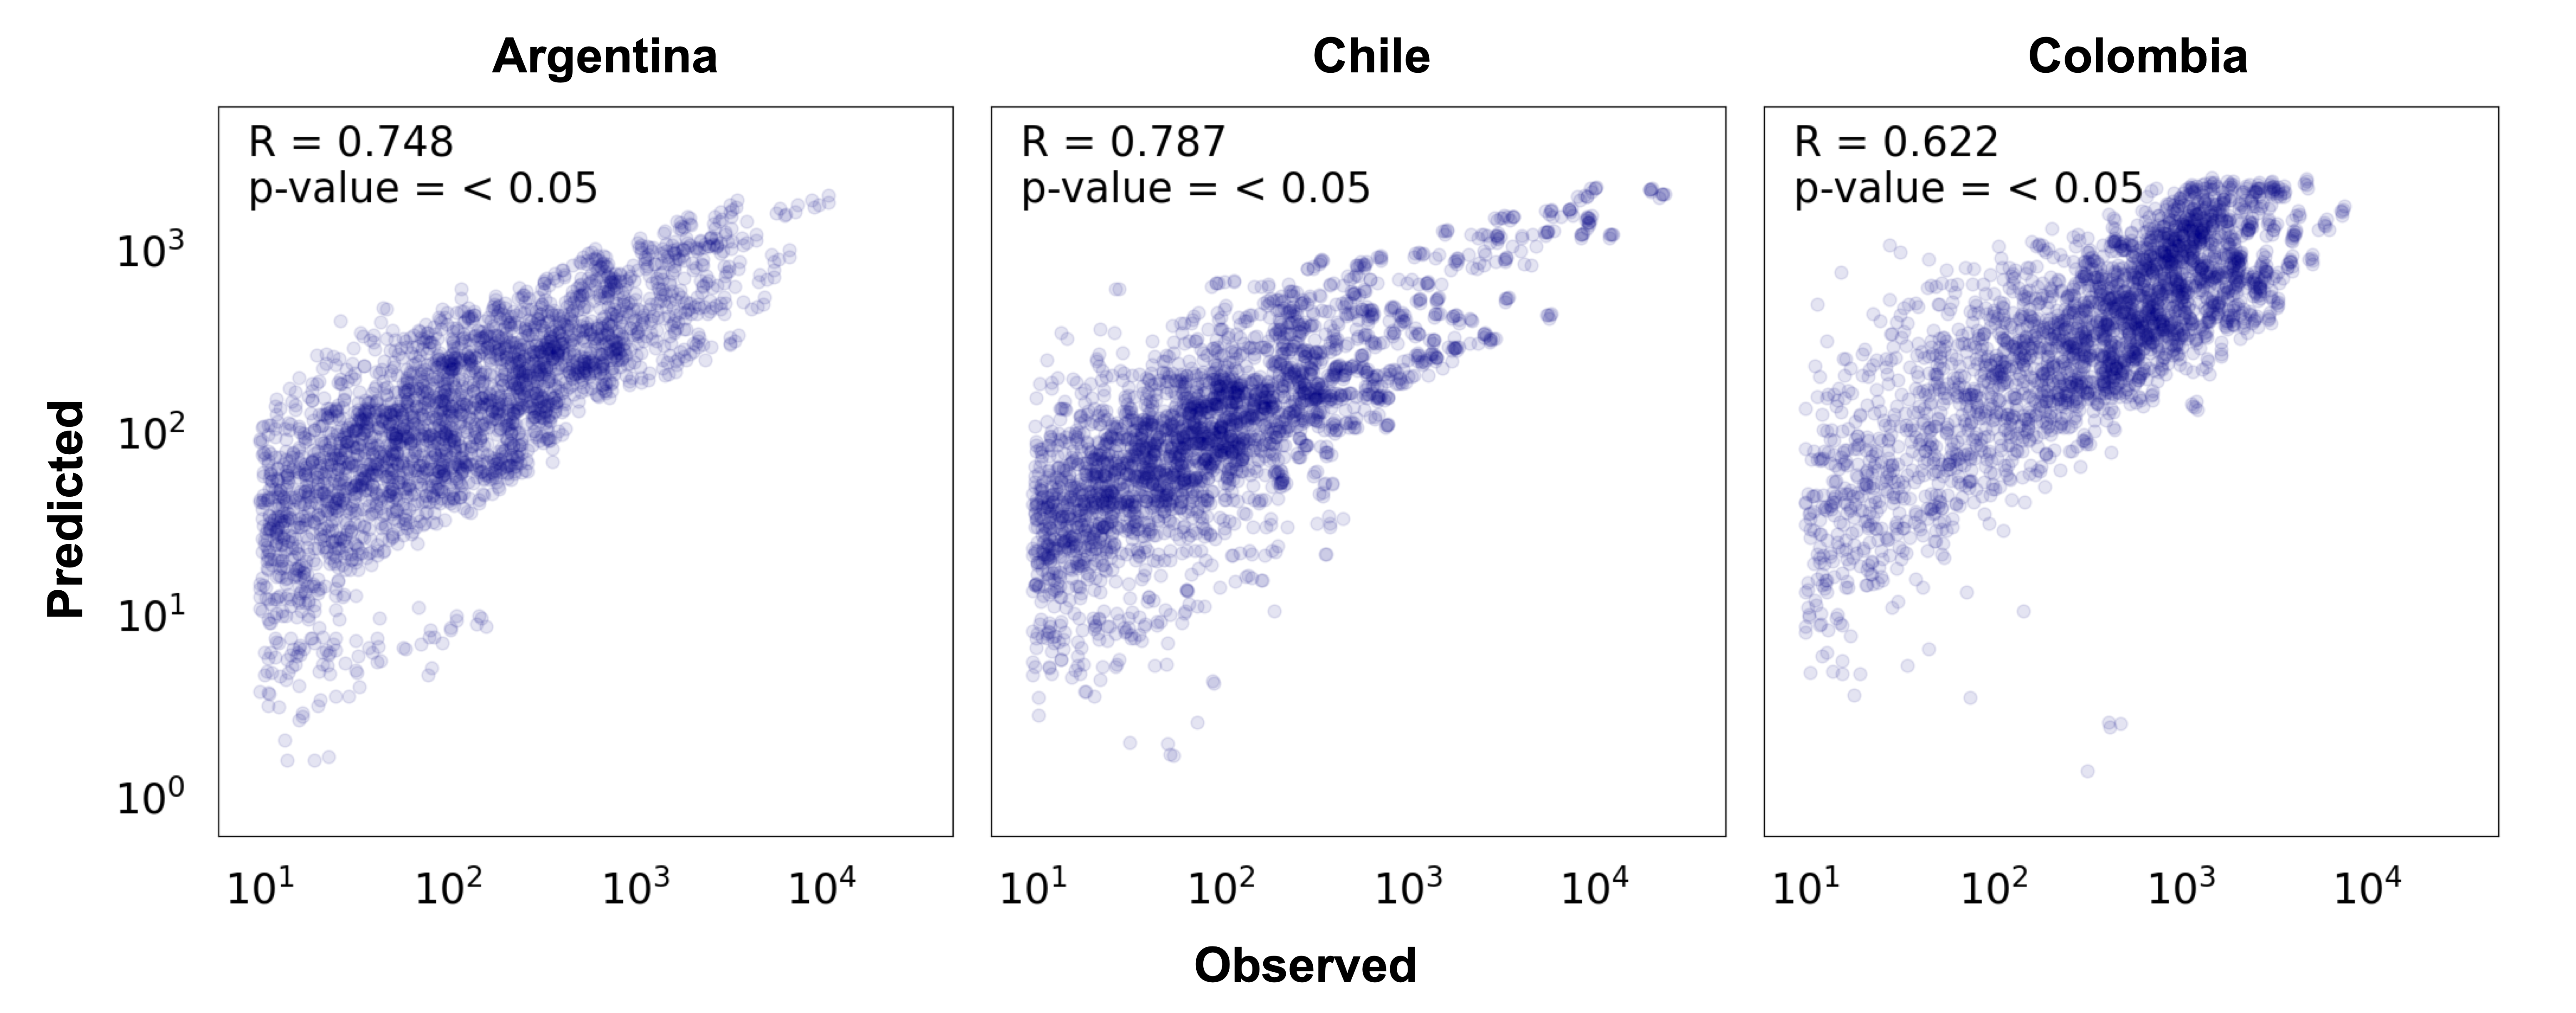
\includegraphics[width=\linewidth]{supplementary/sim/SF-sim-validation.png}
\caption{Relationship between observed and predicted value of number of movements between origin-destination pairs of Bing tiles during the baseline, for all weekdays.}
\end{figure}

\begin{figure}[h!]
\centering
\includegraphics[width=\linewidth]{supplementary/sim/SF-sim-check.png}
\caption{Relationship between Facebook Population at the origin and the destination of each population flow during the baseline period. The Facebook Population is considered after the imputation of the Facebook Population baseline data. The colour of the markers represents the volume of the flows during the baseline period, both observed and predicted through the spatial interaction model. Note that the Bing tiles used to record Facebook Movement data in Colombia are smaller than in Argentina and Chile, hence the lower numbers. }
\end{figure}


\newpage
\section{Classification of tiles according to level of urbanisation and socioeconomic deprivation}

\begin{figure}[h!]
\centering
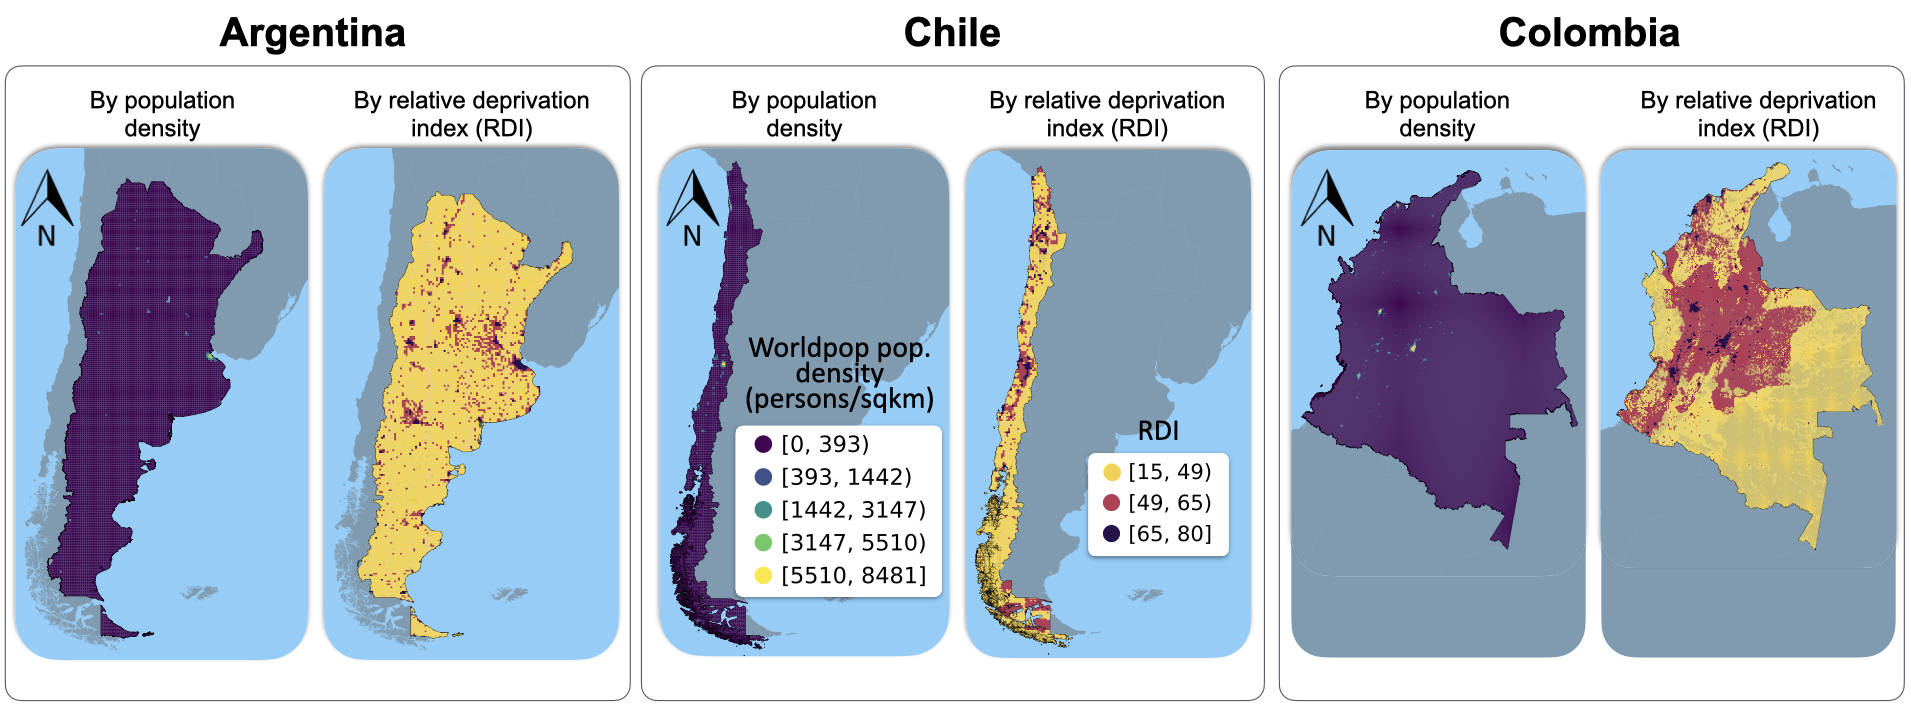
\includegraphics[width=\linewidth]{supplementary/categories/SF-maps-classes-r1.png}
\caption{Classification of spatial units into categories by population density and by relative deprivation index. This figure provides descriptive context for the key socioeconomic and density categories used in the analysis.}
\end{figure}

\begin{figure}[h!]
\centering
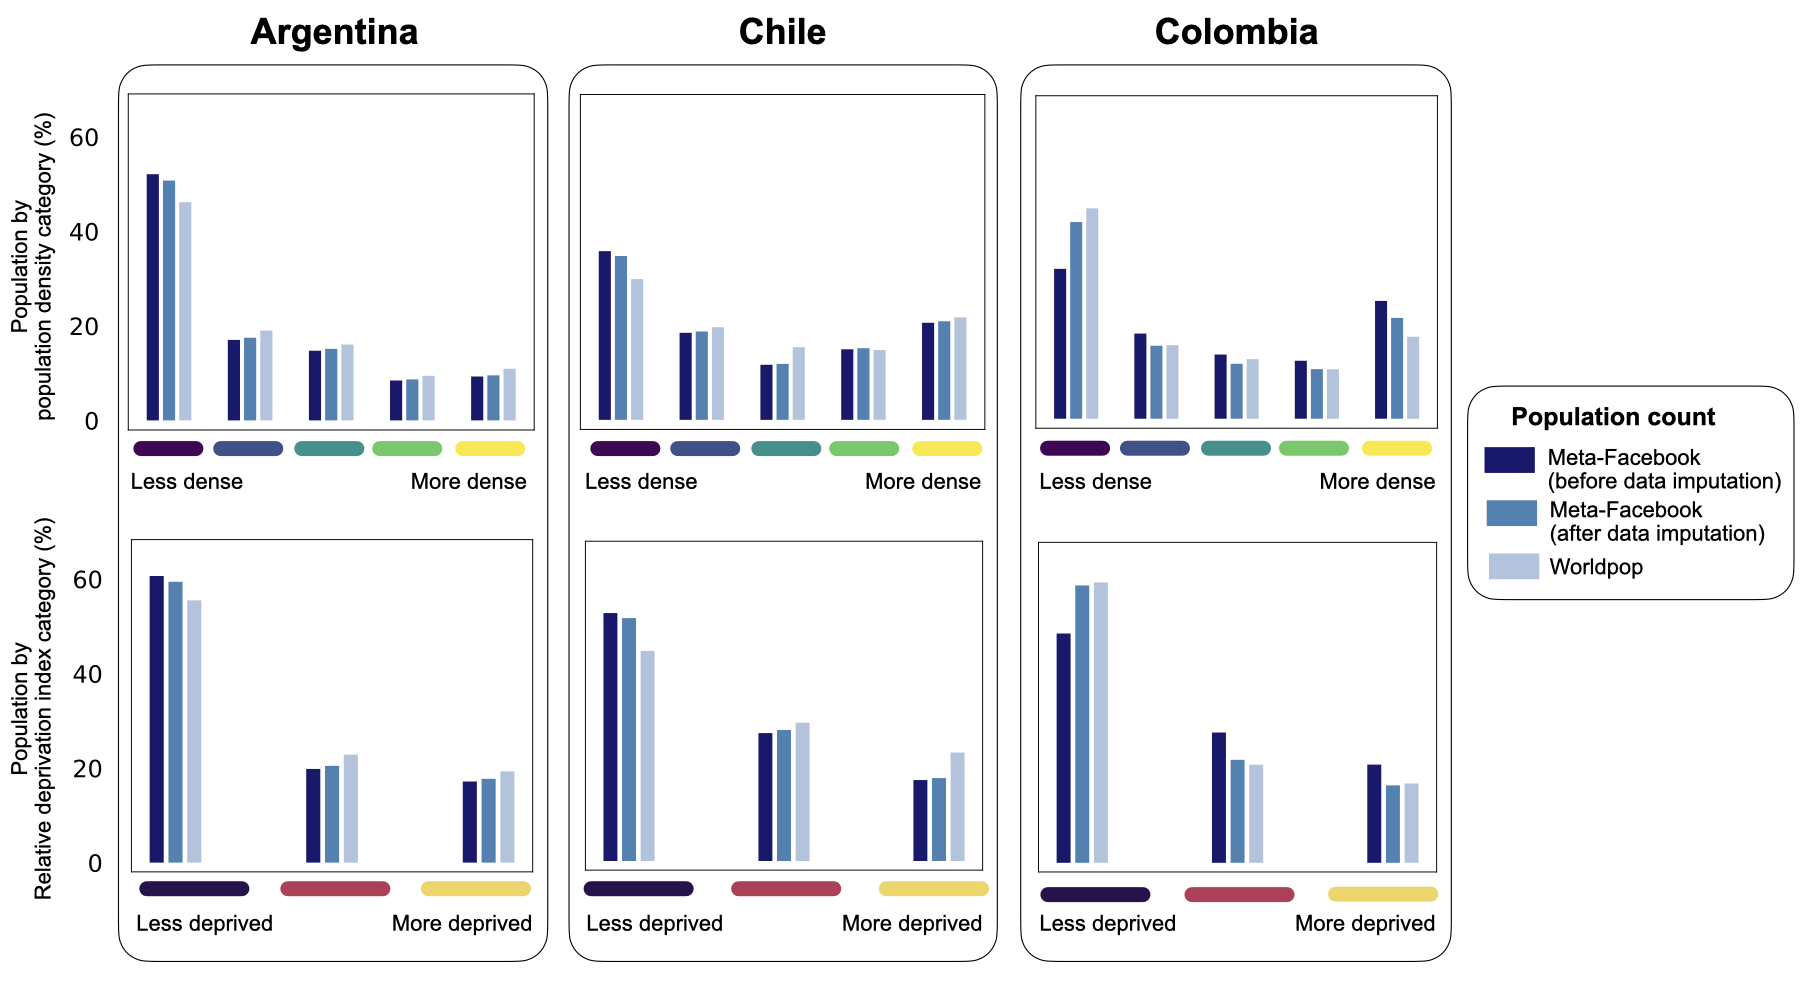
\includegraphics[width=\linewidth]{supplementary/categories/SF-classes-bias-r1.png}
\caption{Population share in each population density and Relative Deprivation Index category by country, according to Meta-Facebook data (before and after imputation) and to Worldpop data. The similarity in category-specific population shares across the Facebook and Worldpop indicates that the Meta-Facebook data provide reasonably representative coverage across deprivation categories, particularly after imputation.}
\end{figure}

\begin{figure}[h!]
\centering
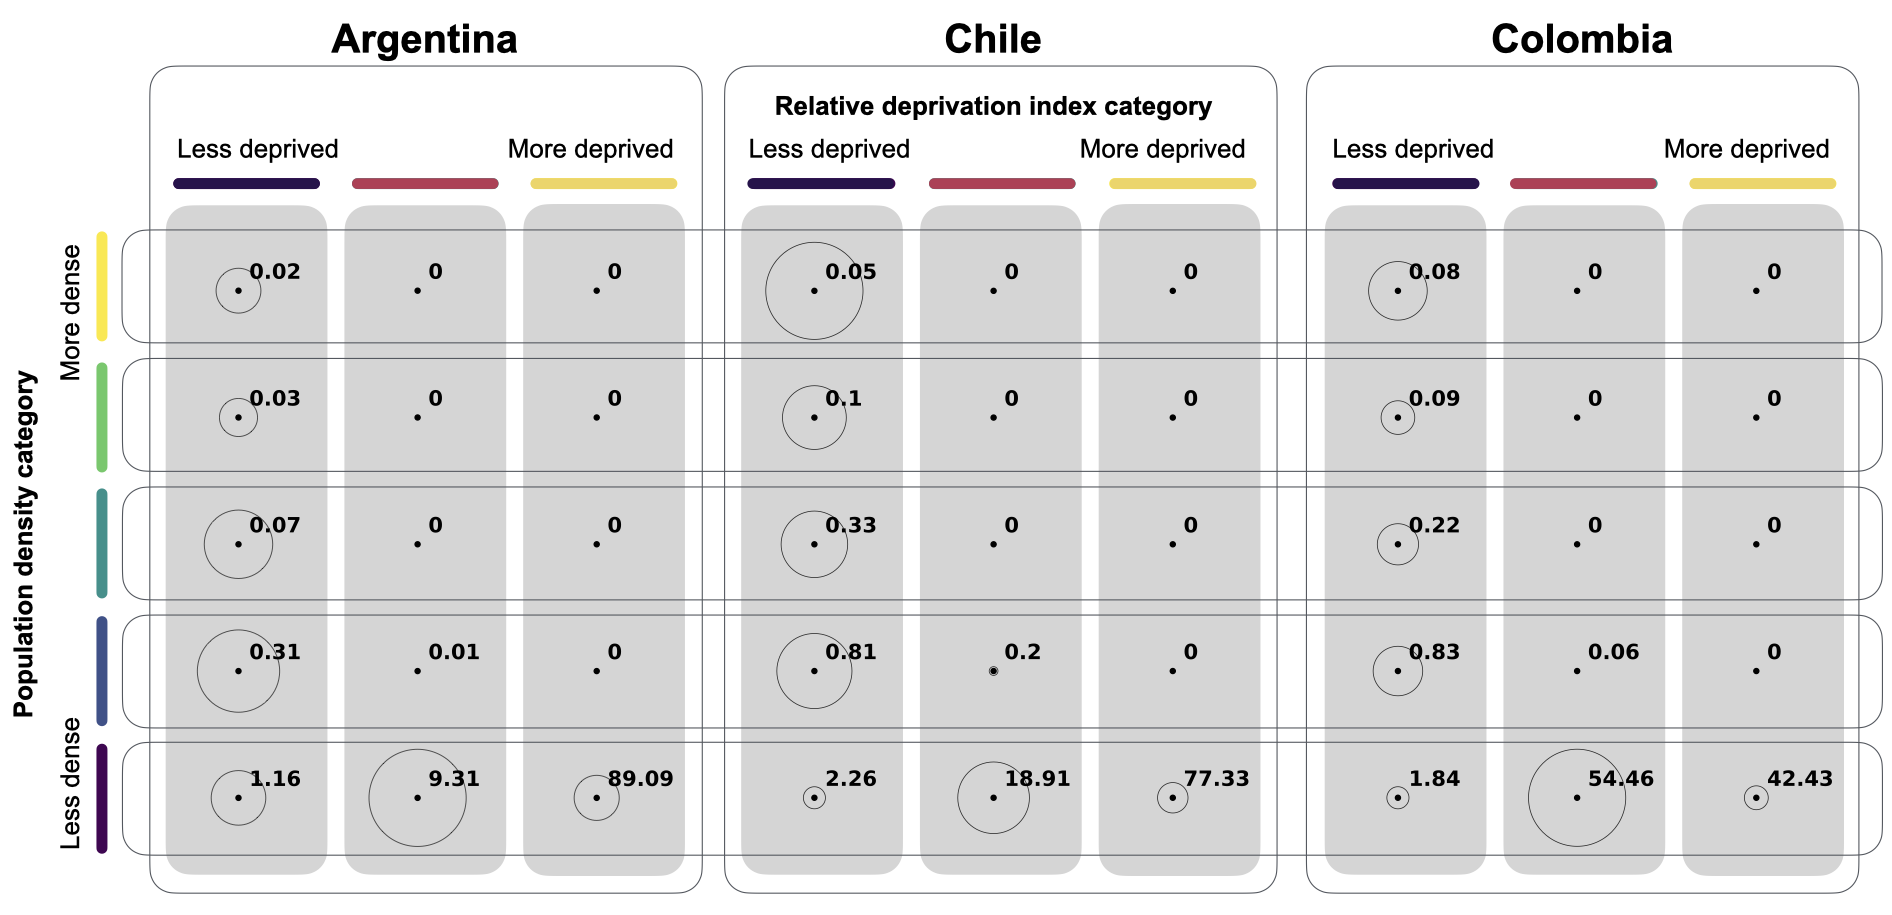
\includegraphics[width=\linewidth]{supplementary/categories/SF-classes-combined-r1.png}
\caption{Joint distribution of spatial units by population density (rows) and relative deprivation index (RDI) categories (columns), with values representing the percentage of spatial units within each country. Circle sizes indicate the total population corresponding to each category pair. This figure provides descriptive context for the combined socioeconomic and density structure of the study areas.}
\end{figure}

\clearpage
\section{Trend analysis}

\subsection{Time series to be modelled with trend analysis}

\begin{figure}[h!]
\centering
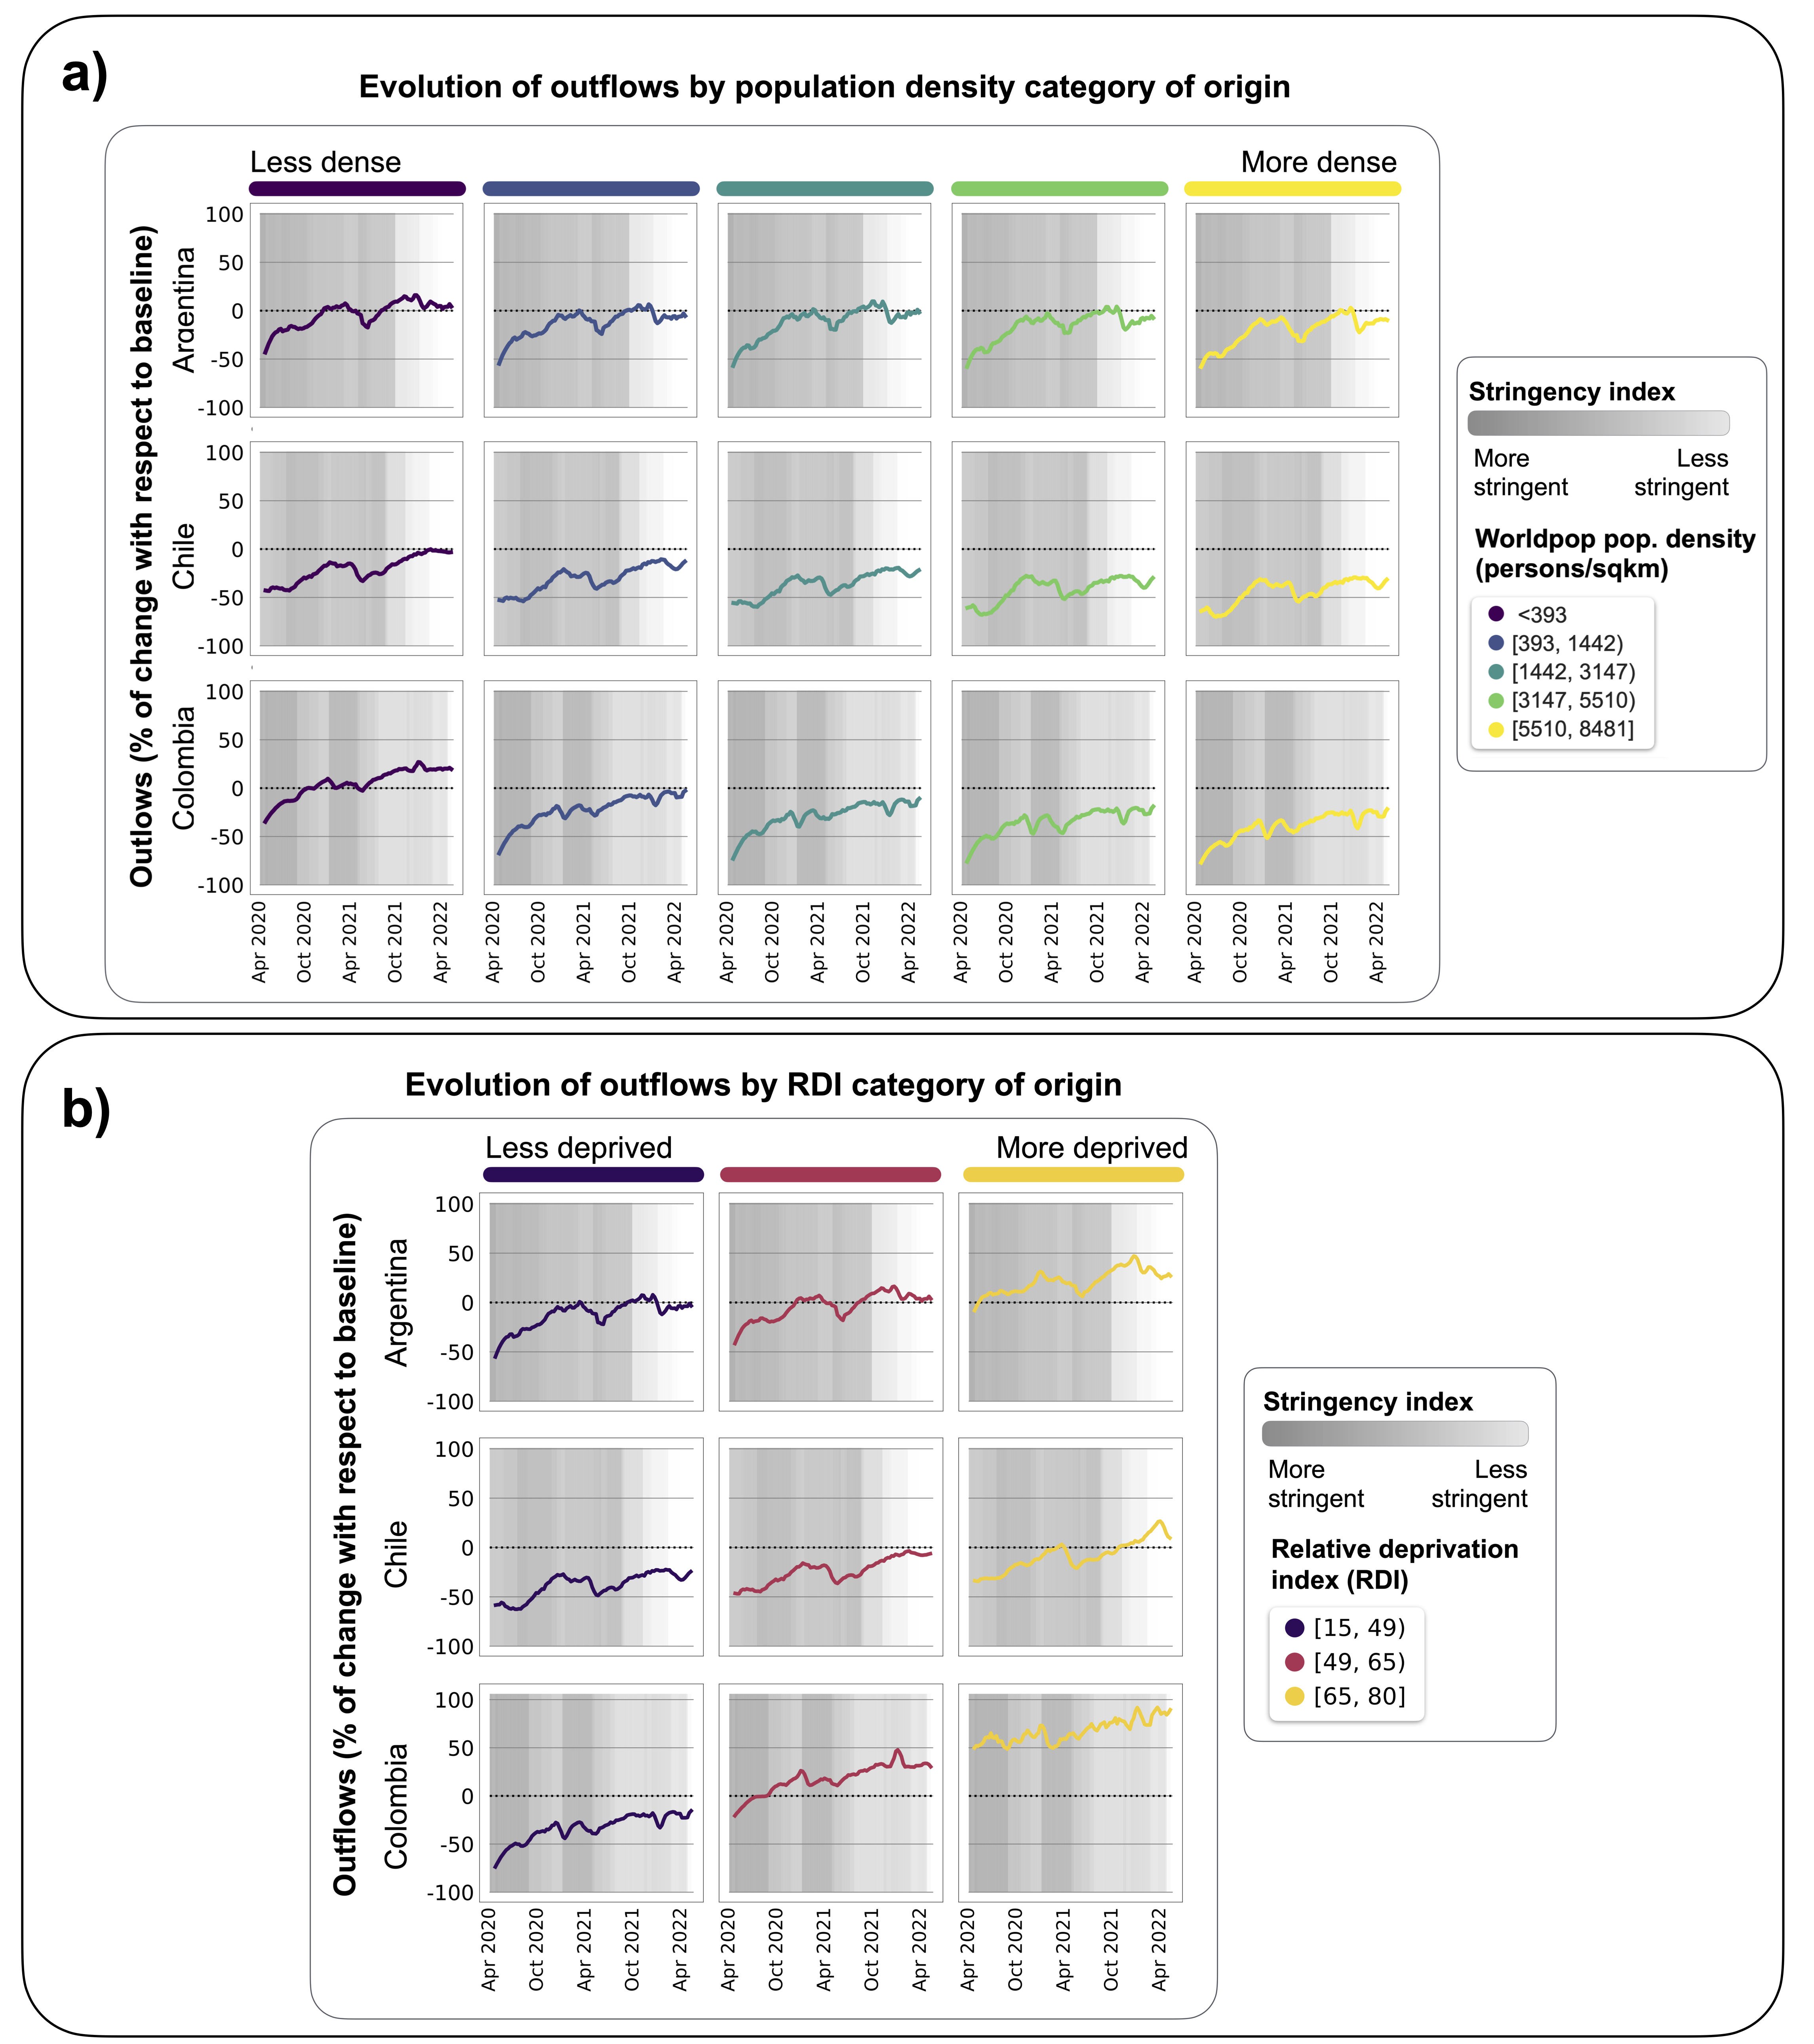
\includegraphics[width=0.8\linewidth]{supplementary/time-series/Fig-recovery-combined-design-r1.png}
\caption{Time evolution of percentage change of outflows relative to pre-pandemic baseline levels, by country and by (a) population density category and (b) relative deprivation category.}
\label{fig-classification}
\end{figure}

\clearpage
\subsection{Robustness of trend extraction method}

\begin{table}[h!]
\centering
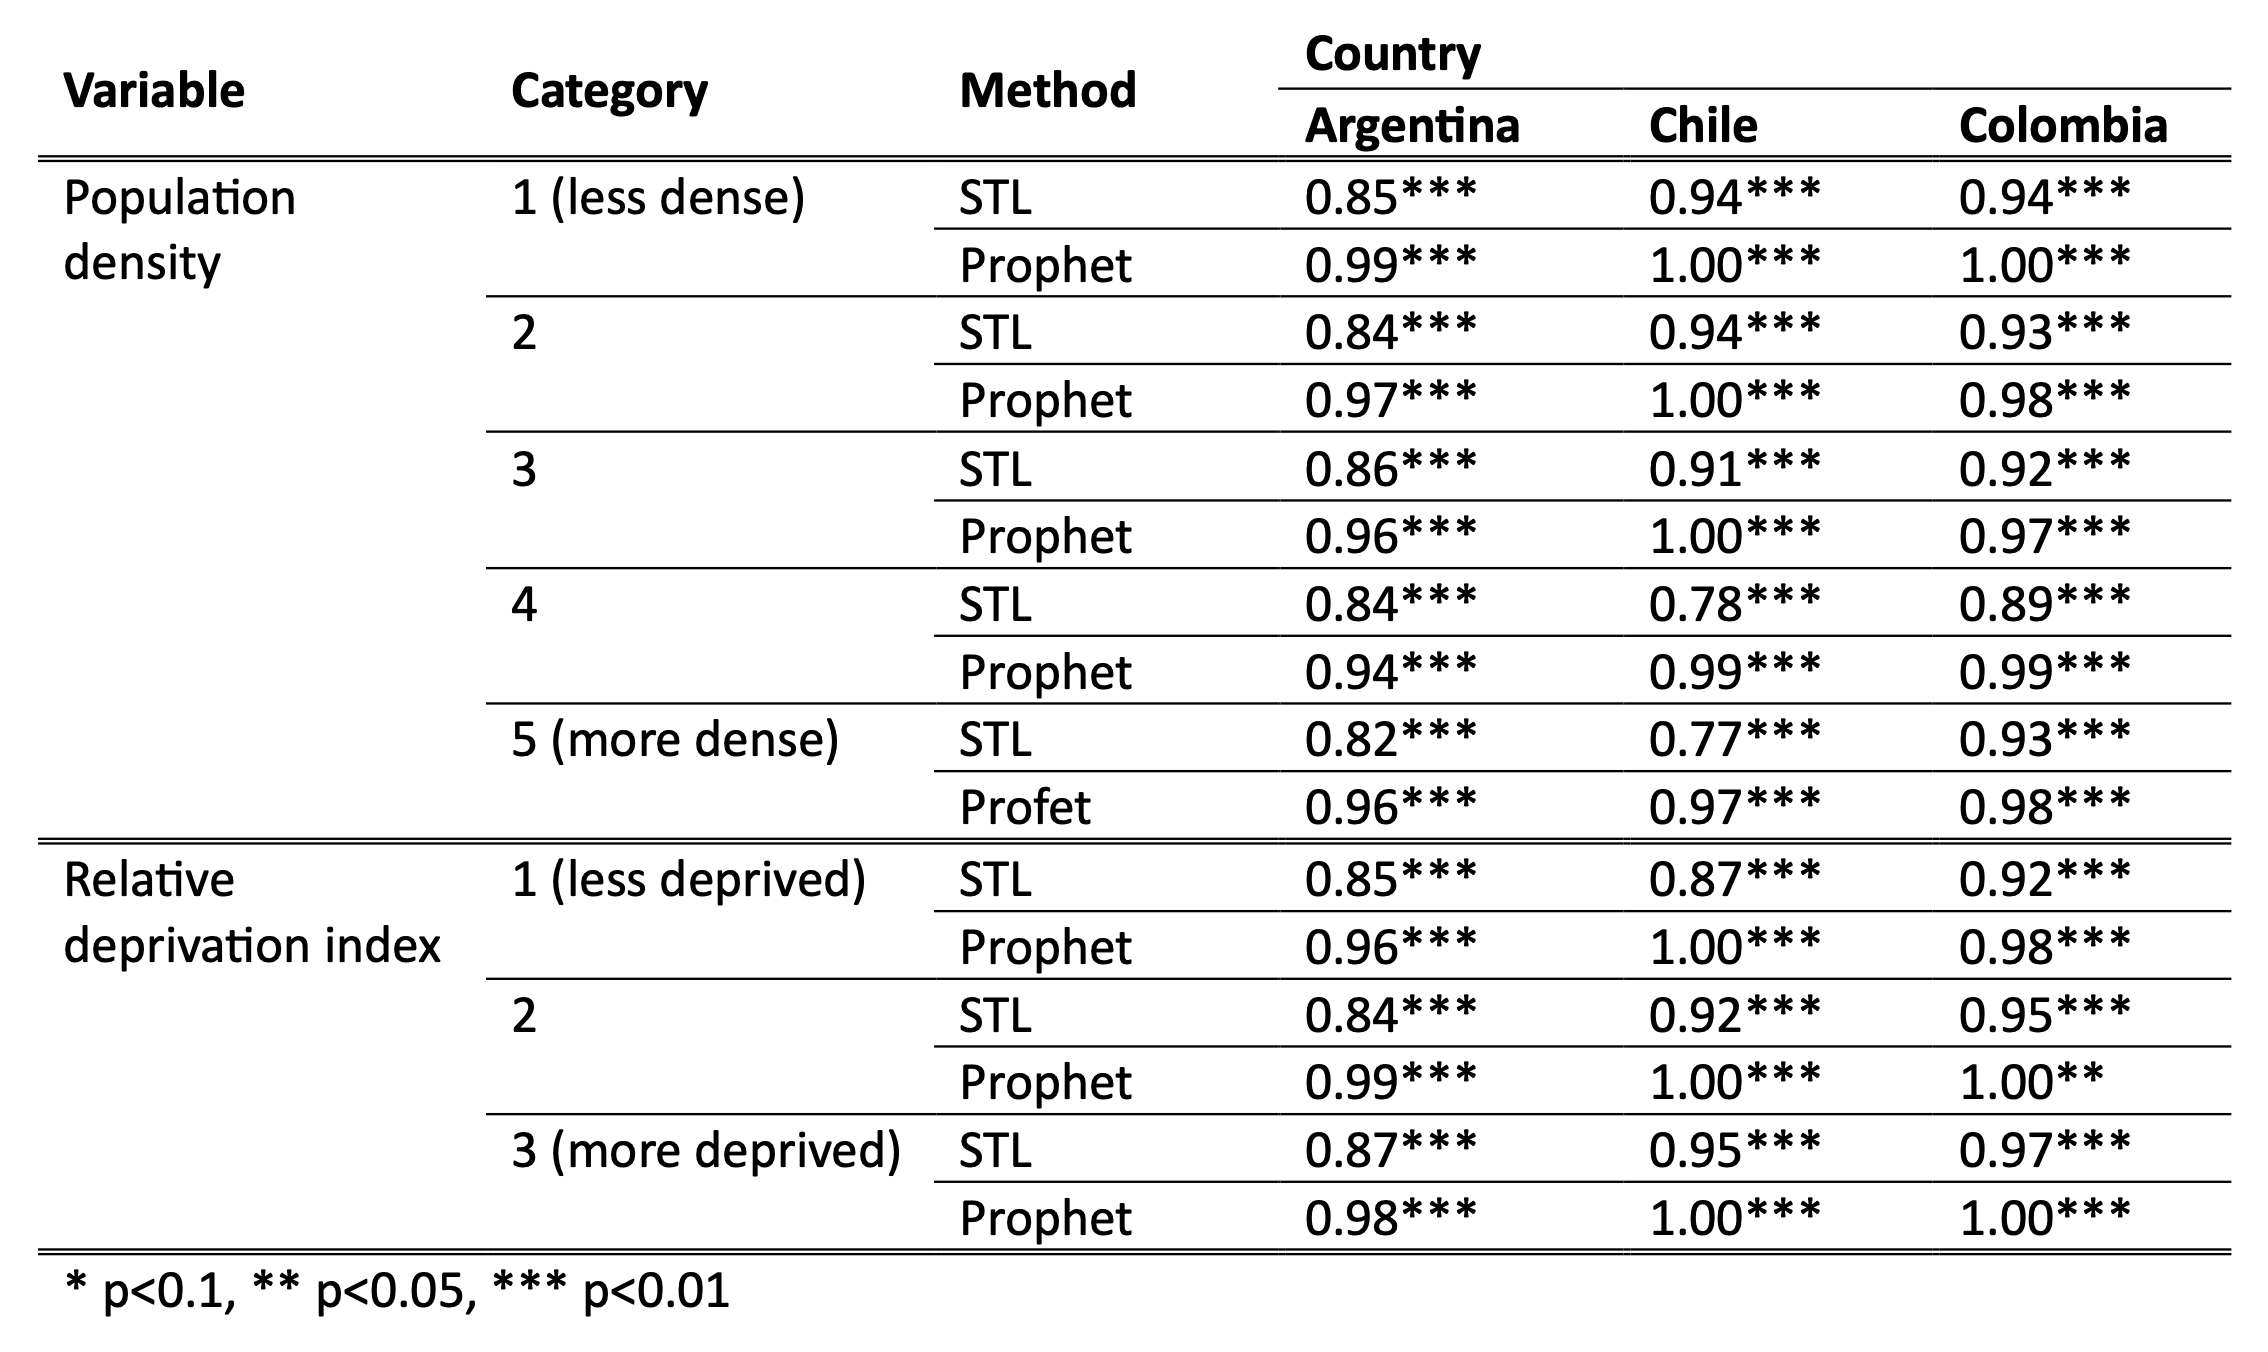
\includegraphics[width=0.8\linewidth]{supplementary/trend-extraction/trend-extraction-robustness-r1.png}
\caption{Pearson correlation coefficients (with p-values) comparing trends extracted using the moving-average method (used in the main analysis) with those extracted using Seasonal-Trend decomposition using Loess (STL) decomposition and the Prophet model. Results are reported for each country and across all population density and relative deprivation categories. The high correlations indicate strong consistency across trend extraction methods.}
\end{table}


\subsection{Model specification}

\begin{table}[h!]
\centering
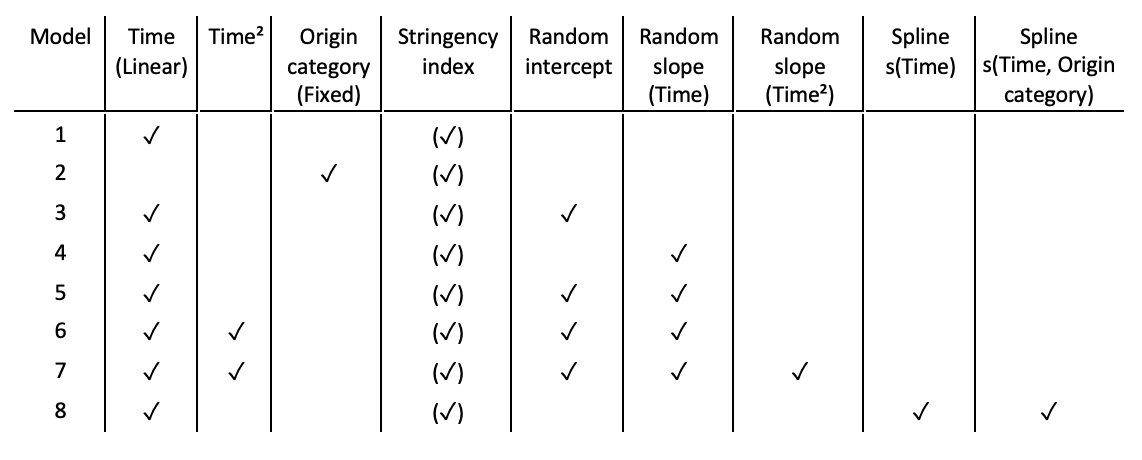
\includegraphics[width=0.8\linewidth]{supplementary/models-tables/SF-models-specification.png}
\caption{Summary of model specifications. There is a total of 16: 14 for mixed-effects, 2 for Generalised Additive Models with spline terms. Each row in the table represents a pair of models: one that includes the stringency index as a covariate and one that excludes it. This is denoted by a bracketed check mark [(\checkmark)]. All other check marks [\checkmark] indicate terms that are included in both models of the pair. Random effects and the second spline term are considered according to the population density or the Relative Deprivation Index (RDI) of the origin location of outflows.}
\end{table}



\newpage
\subsection{Mixed-effects model outcomes by old-age dependency ratio categories}

\begin{figure}[h!]
\centering
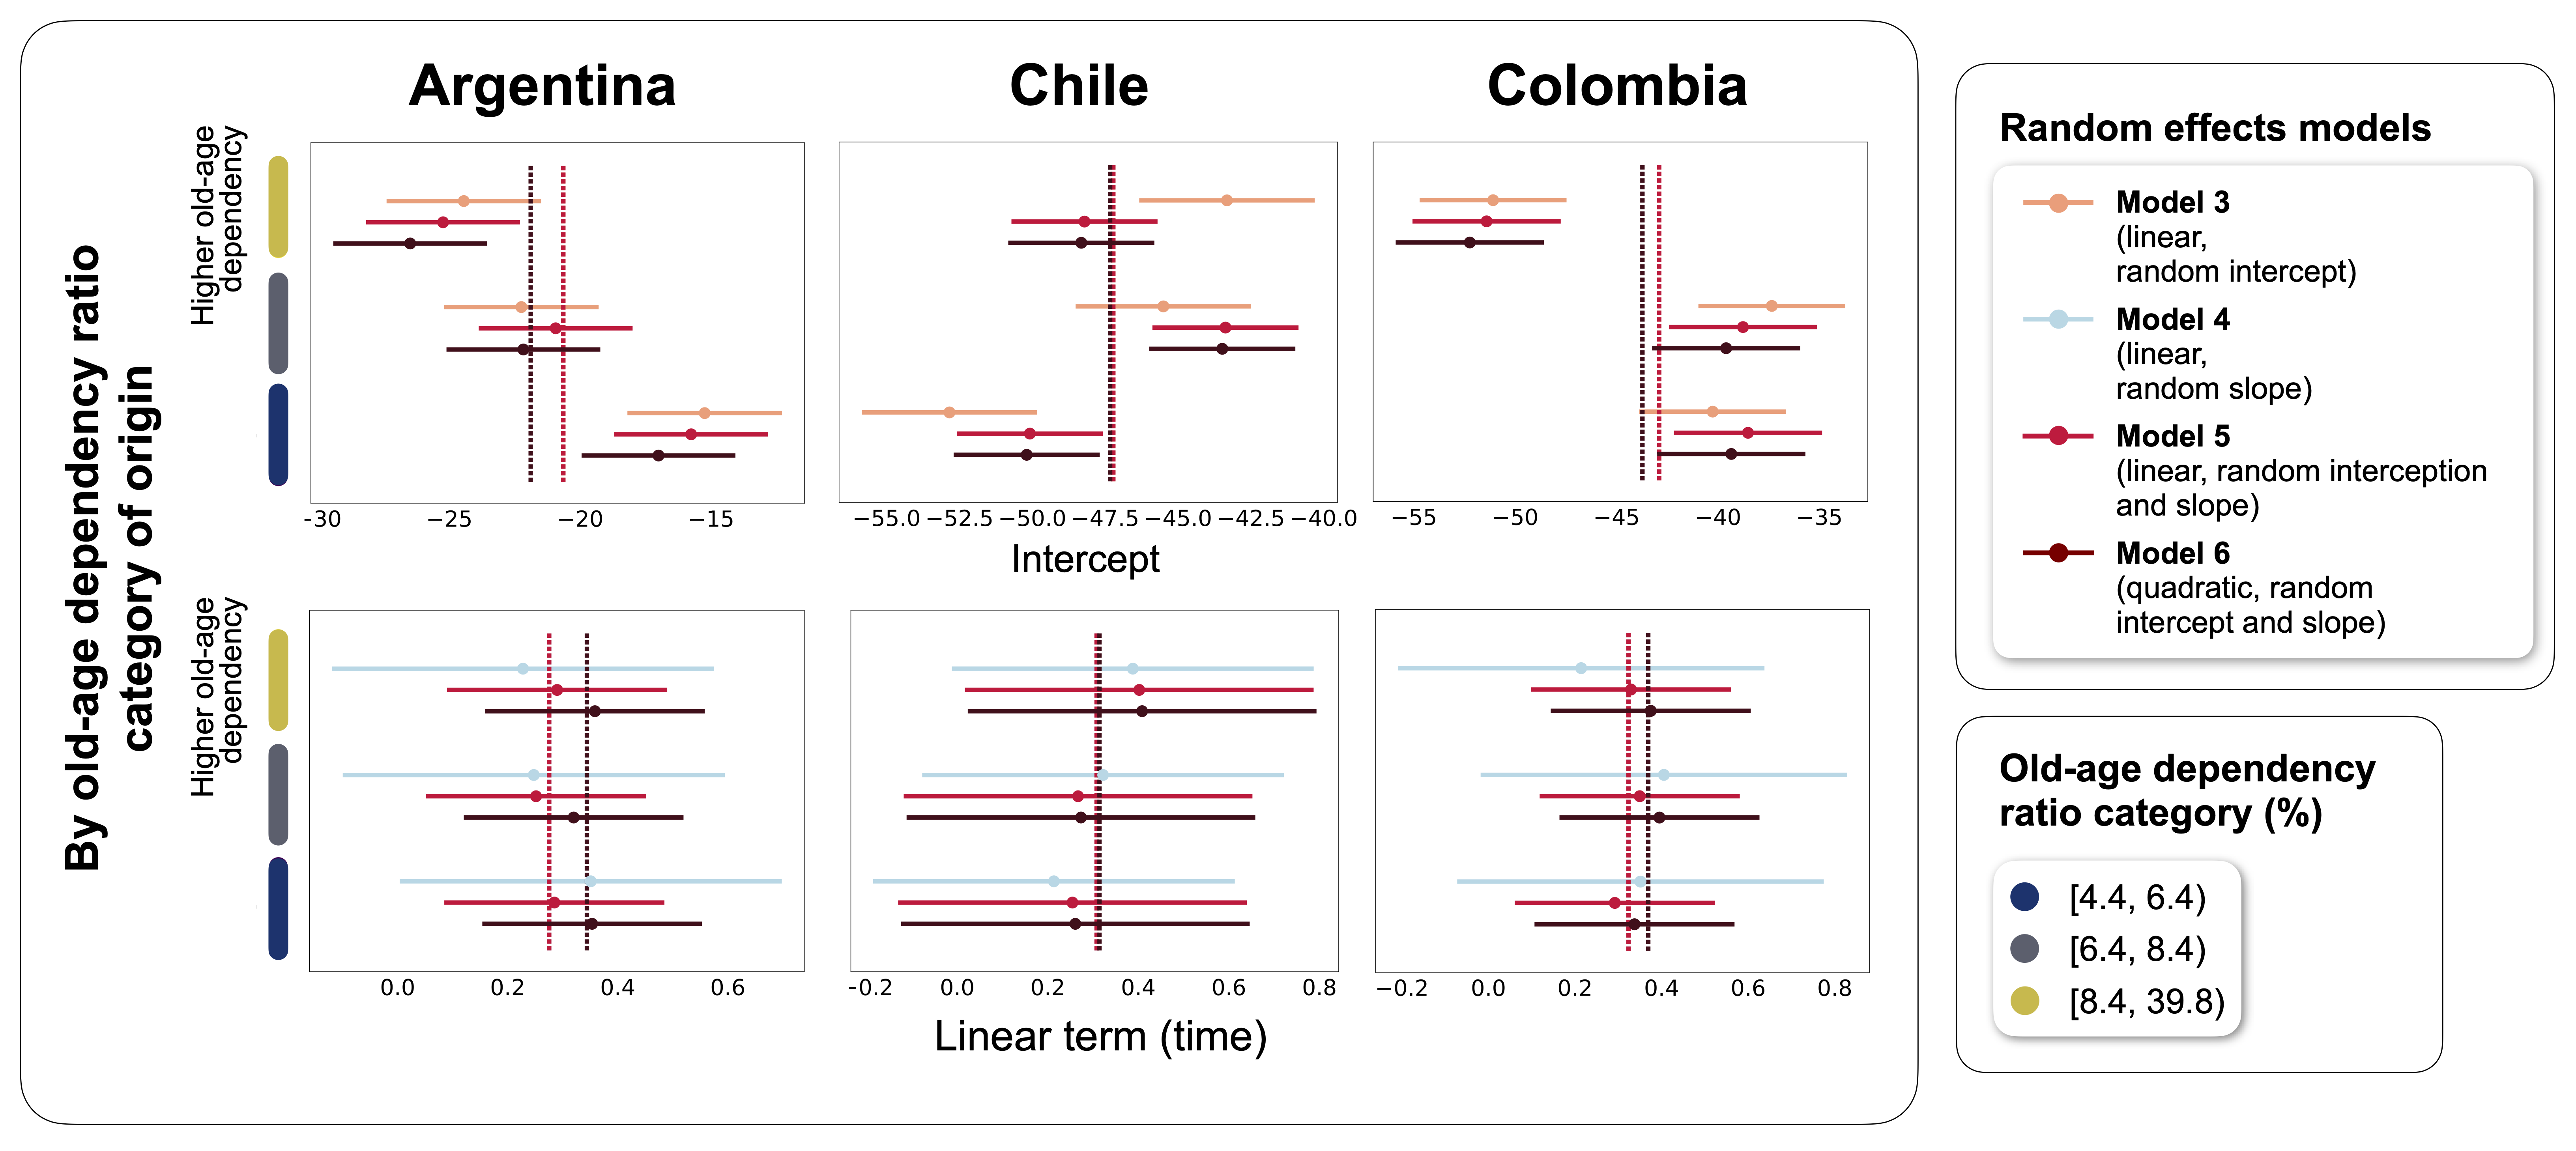
\includegraphics[width=\linewidth]{supplementary/models-figures/SF-re-combined-design-oldage-r1.png}
\caption{Mixed-effects modelling estimates (random intercept and random
linear time term), by country and old-age dependency ratio category; bars denote 95\% confidence intervals; colours encode different model specifications; vertical dashed lines
represent the estimated values for fixed effects of the corresponding terms (i.e. intercept, linear time). Panel a) displays results by population density category and b) by relative
deprivation category.}
\end{figure}

\clearpage
\subsection{Model estimates - relative change in outflows}

\begin{table}[h!]
\centering
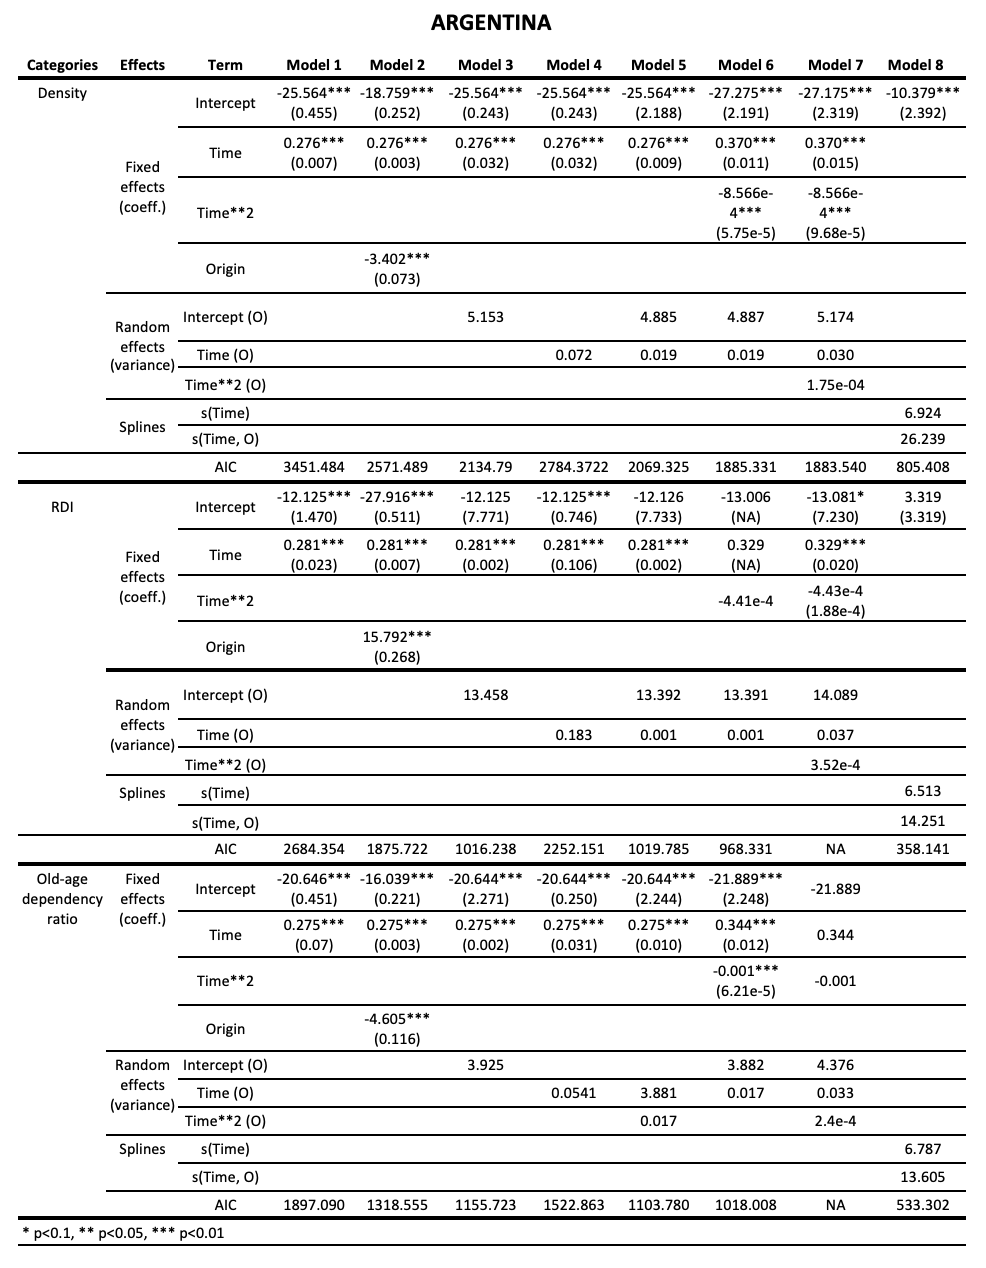
\includegraphics[width=0.9\linewidth]{supplementary/models-tables/models-table-ARG-quadratic-new-r1.png}
\caption{Results of mixed-effects and Generalised Additive Model (GAM) models for trend analysis of relative change in outflows in Argentina. Fixed and random effects according to the population density, the Relative Deprivation Index (RDI) or the old-age dependency ratio of the origin location of outflows are reported for Models 1-7. Effective degrees of freedom are reported for the Spline terms in Model 8.}
\end{table}

\clearpage

\begin{table}[h!]
\centering
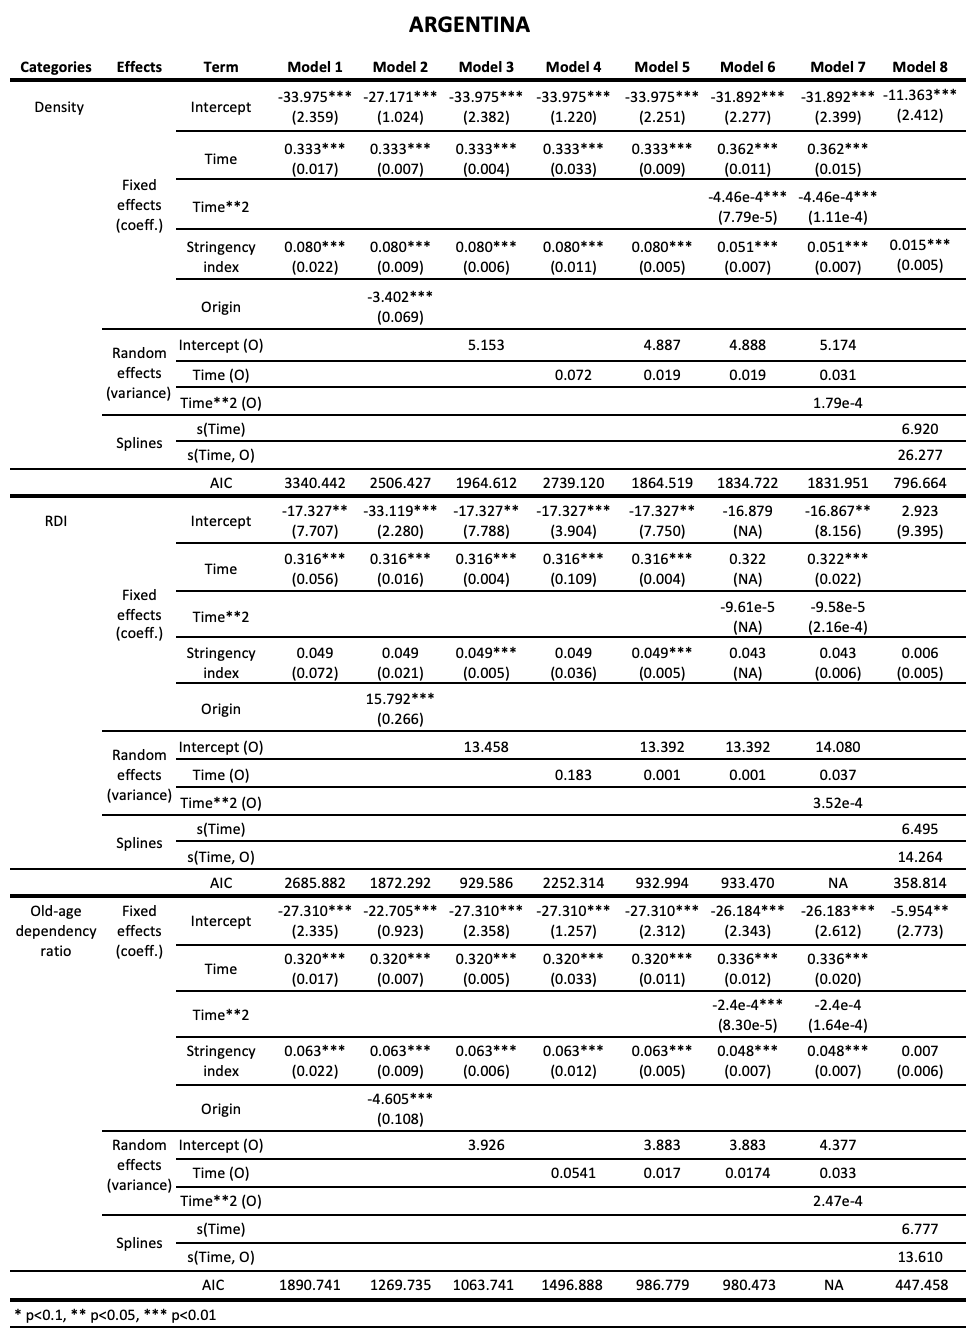
\includegraphics[width=0.9\linewidth]{supplementary/models-tables/models-table-ARG-quadratic-stringenty-new-r1.png}
\caption{Results of mixed-effects and Generalised Additive Model (GAM) models for trend analysis of relative change in outflows in Argentina including stringency index as a predictor variable. Fixed and random effects according to the population density, the Relative Deprivation Index (RDI) or the old-age dependency ratio of the origin location of outflows are reported for Models 1-7. Effective degrees of freedom are reported for the Spline terms in Model 8.}
\label{tab-modelsARG-stringency}
\end{table}

\clearpage

\begin{table}[h!]
\centering
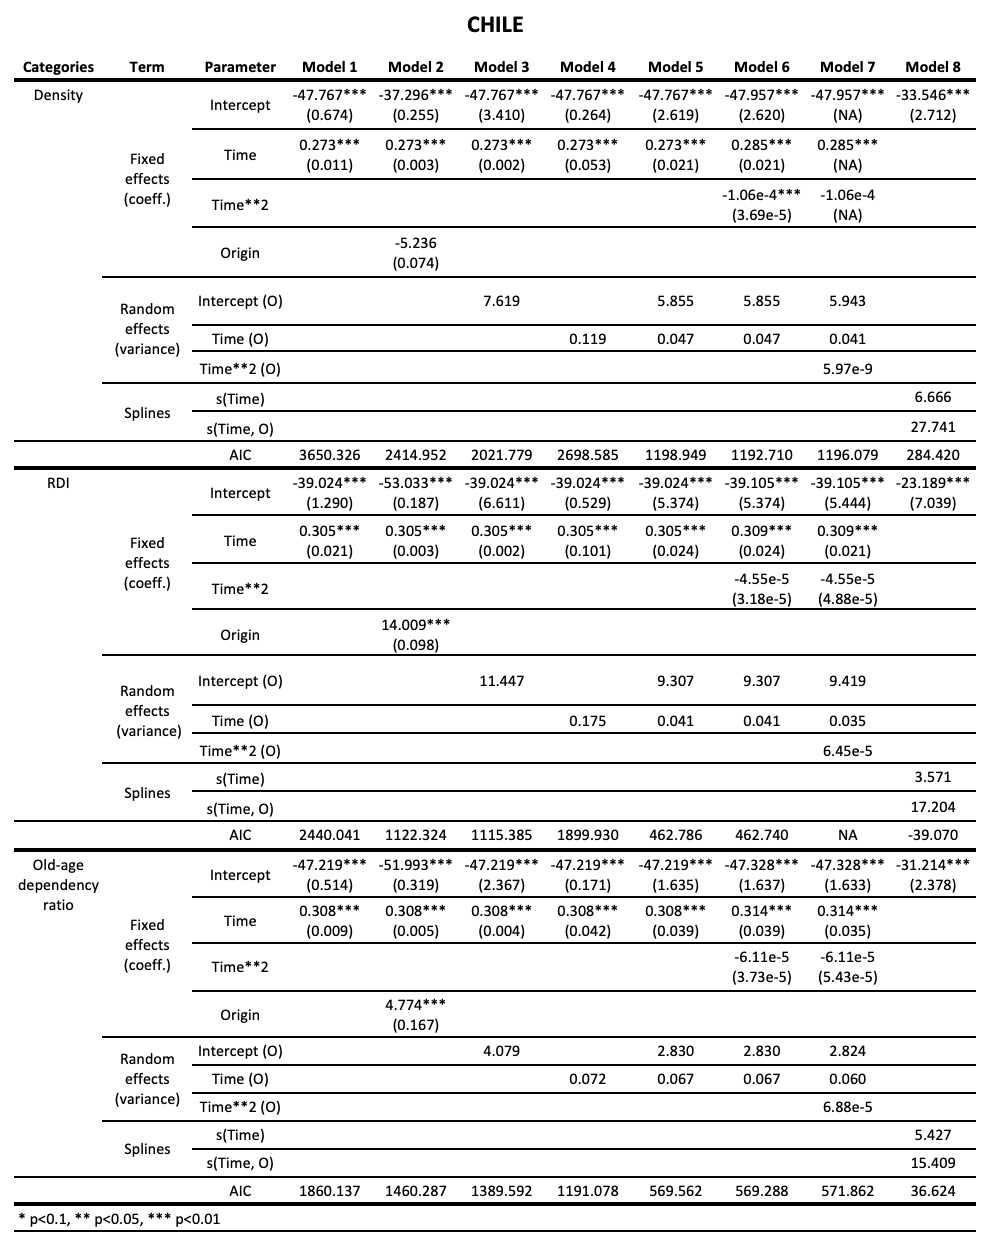
\includegraphics[width=0.9\linewidth]{supplementary/models-tables/models-table-CHL-quadratic-new-r1.png}
\caption{Results of mixed-effects and Generalised Additive Model (GAM) models for trend analysis of relative change in outflows in Chile. Fixed and random effects according to the population density, the Relative Deprivation Index (RDI) or the old-age dependency ratio of the origin location of outflows are reported for Models 1-7. Effective degrees of freedom are reported for the Spline terms in Model 8.}
\label{tab-modelsCHL}
\end{table}

\clearpage

\begin{table}[h!]
\centering
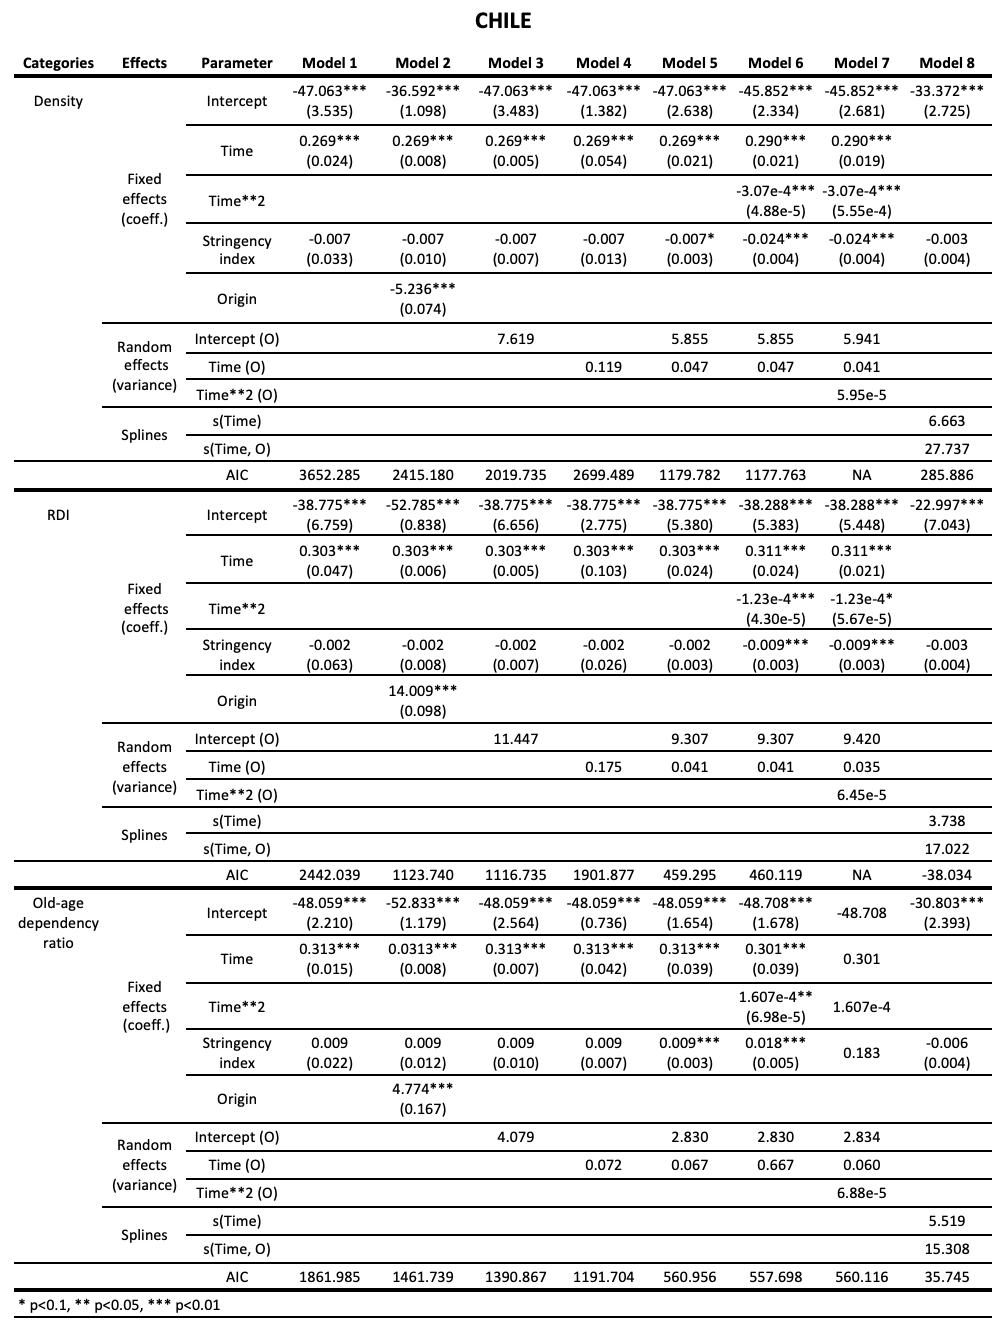
\includegraphics[width=0.9\linewidth]{supplementary/models-tables/models-table-CHL-quadratic-stringency-new-r1.png}
\caption{Results of mixed-effects and Generalised Additive Model (GAM) models for trend analysis of relative change in outflows in Chile including stringency index as a predictor variable. Fixed and random effects according to the population density, the Relative Deprivation Index (RDI) or the old-age dependency ratio of the origin location of outflows are reported for Models 1-7. Effective degrees of freedom are reported for the Spline terms in Model 8.}
\label{tab-modelsCHL-stringency}
\end{table}

\clearpage

\begin{table}[h!]
\centering
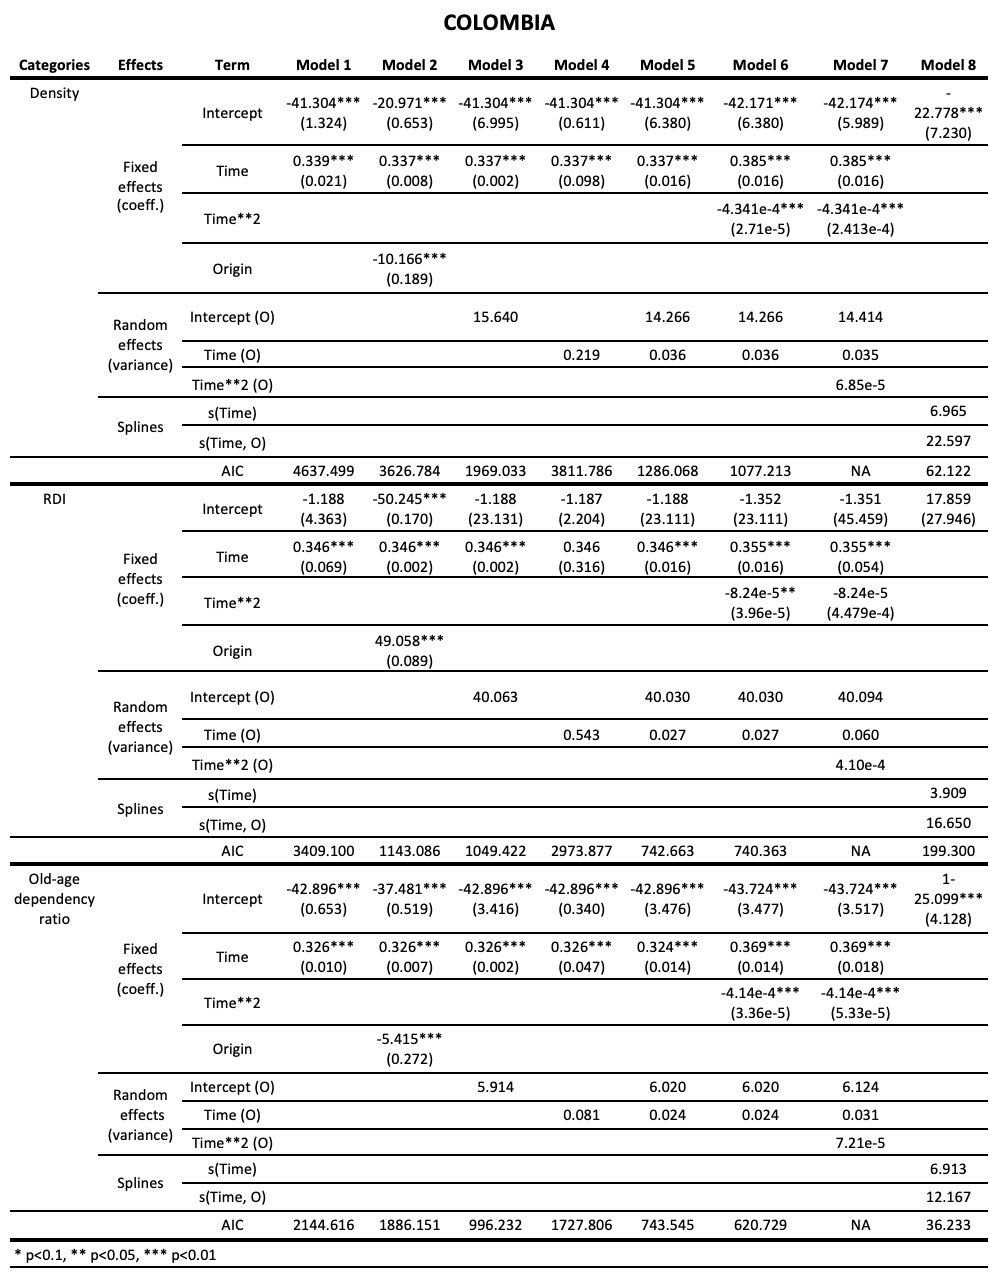
\includegraphics[width=0.9\linewidth]{supplementary/models-tables/models-table-COL-quadratic-new-r1.png}
\caption{Results of mixed-effects and Generalised Additive Model (GAM) models for trend analysis of relative change in outflows in Colombia. Fixed and random effects according to the population density, the Relative Deprivation Index (RDI) or the old-age dependency ratio of the origin location of outflows are reported for Models 1-7. Effective degrees of freedom are reported for the Spline terms in Model 8.}
\label{tab-modelsCOL}
\end{table}

\clearpage

\begin{table}[h!]
\centering

\includegraphics[width=0.9\linewidth]{supplementary/models-tables/models-table-COL-quadratic-stringency-new-r1.png}
\caption{Results of mixed-effects and Generalised Additive Model (GAM) models for trend analysis of relative change in outflows in Colombia including stringency index as a predictor variable. Fixed and random effects according to the population density, the Relative Deprivation Index (RDI) or the old-age dependency ratio of the origin location of outflows are reported for Models 1-7. Effective degrees of freedom are reported for the Spline terms in Model 8.}
\label{tab-modelsCOL-stringency}
\end{table}

\clearpage

\subsection{Model estimates - relative change in netflows involving capital}

\begin{table}[h!]
\centering
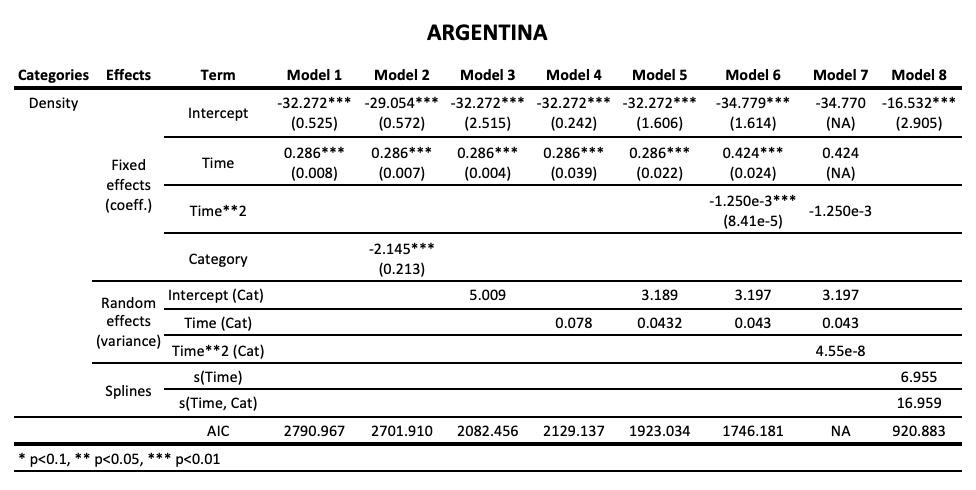
\includegraphics[width=\linewidth]{supplementary/models-tables/models-table-ARG-quadratic-capital-r1.png}
\caption{Results of mixed-effects and Generalised Additive Model (GAM) models for trend analysis of relative change in netflows involving urban region surrounding capital in Argentina. Netflows are defined as inflows to an urban core minus outflows from the urban core. Random effects and spline terms according to population density.}
\label{tab-modelsARG-capital}
\end{table}


\begin{table}[h!]
\centering
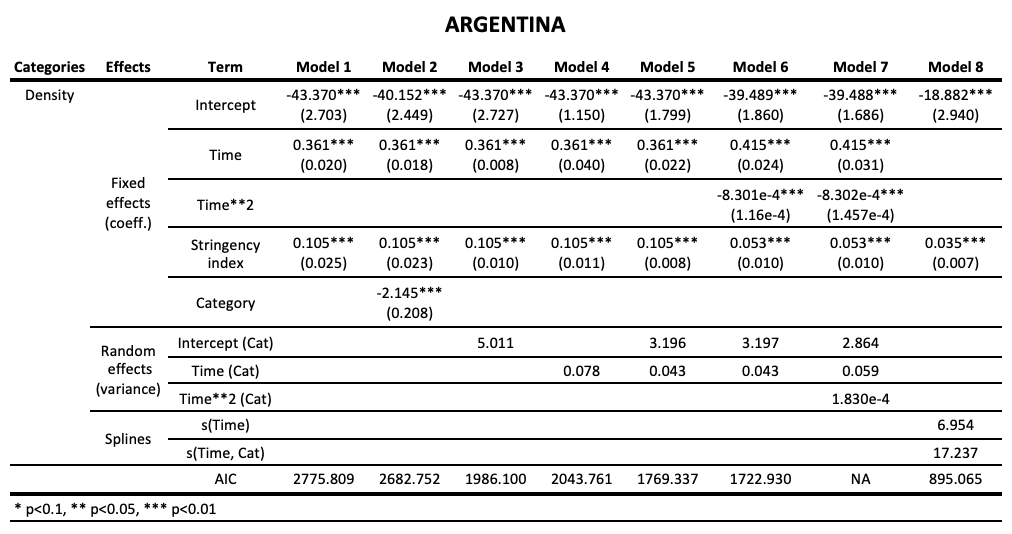
\includegraphics[width=\linewidth]{supplementary/models-tables/models-table-ARG-quadratic-capital-stringency-r1.png}
\caption{Results of mixed-effects and Generalised Additive Model (GAM) models for trend analysis of relative change in netflows involving urban region surrounding capital in Argentina including stringency index as a predictor variable. Netflows are defined as inflows to an urban core minus outflows from the urban core. Random effects and spline terms according to population density.}
\label{tab-modelsARG-capital-stringency}
\end{table}

\newpage

\begin{table}[h!]
\centering
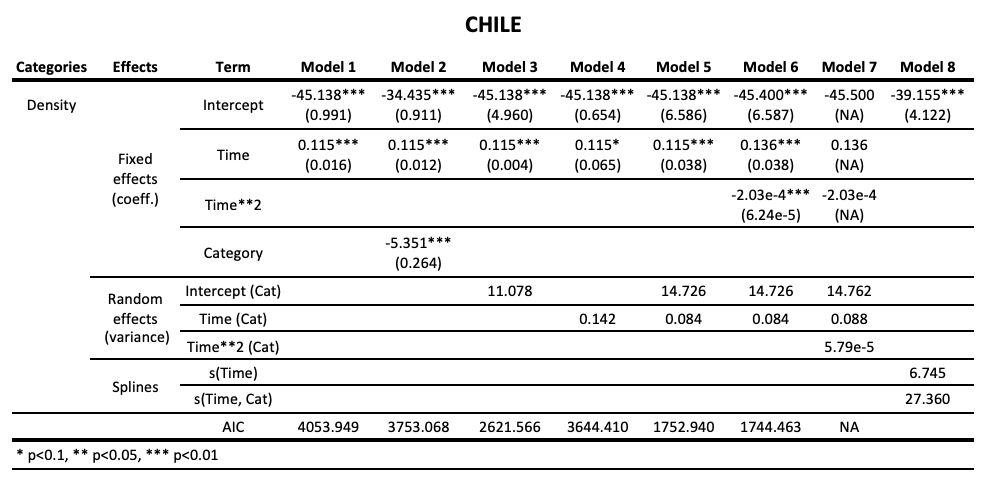
\includegraphics[width=\linewidth]{supplementary/models-tables/models-table-CHL-quadratic-capital-r1.png}
\caption{Results of mixed-effects and Generalised Additive Model (GAM) models for trend analysis of relative change in netflows involving urban region surrounding capital in Chile. Netflows are defined as inflows to an urban core minus outflows from the urban core. Random effects and spline terms according to population density.}
\label{tab-modelsCHL-capital}
\end{table}


\begin{table}[h!]
\centering
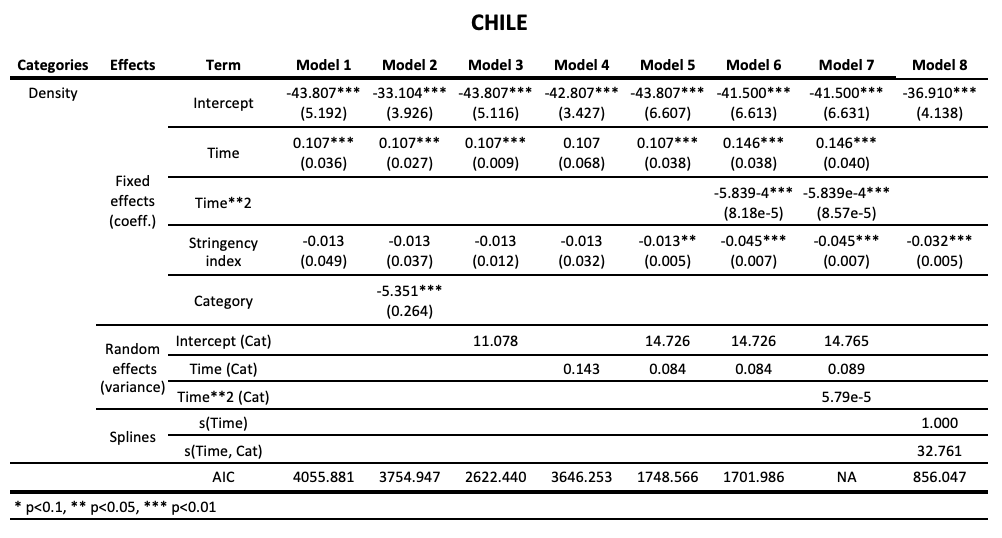
\includegraphics[width=\linewidth]{supplementary/models-tables/models-table-CHL-quadratic-capital-stringency-r1.png}
\caption{Results of mixed-effects and Generalised Additive Model (GAM) models for trend analysis of relative change in netflows involving urban region surrounding capital in Chile including stringency index as a predictor variable. Netflows are defined as inflows to an urban core minus outflows from the urban core. Random effects and spline terms according to population density.}
\label{tab-modelsCHL-capital-stringency}
\end{table}

\newpage

\begin{table}[h!]
\centering
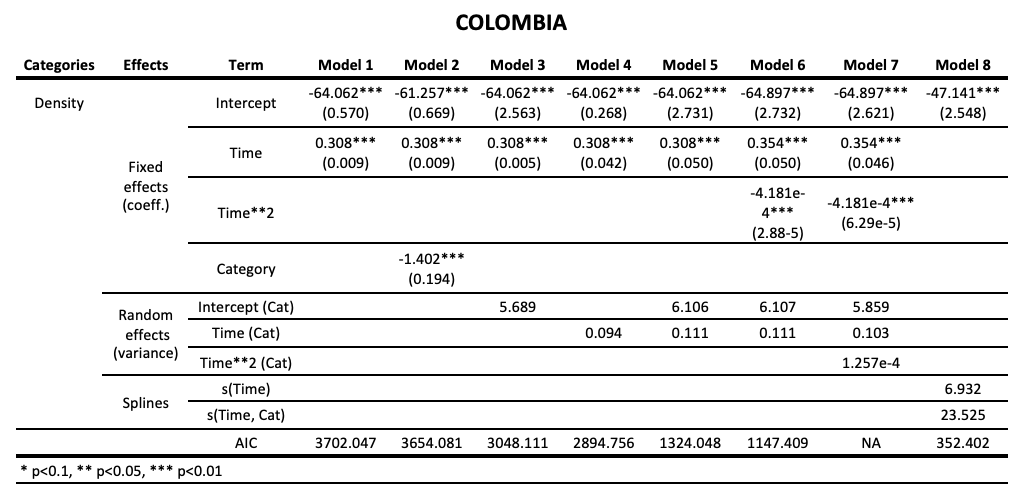
\includegraphics[width=\linewidth]{supplementary/models-tables/models-table-COL-quadratic-capital-r1.png}
\caption{Results of mixed-effects and Generalised Additive Model (GAM) models for trend analysis of relative change in netflows involving urban region surrounding capital in Colombia. Netflows are defined as inflows to an urban core minus outflows from the urban core. Random effects and spline terms according to population density.}
\label{tab-modelsCOL-capital}
\end{table}

\begin{table}[h!]
\centering
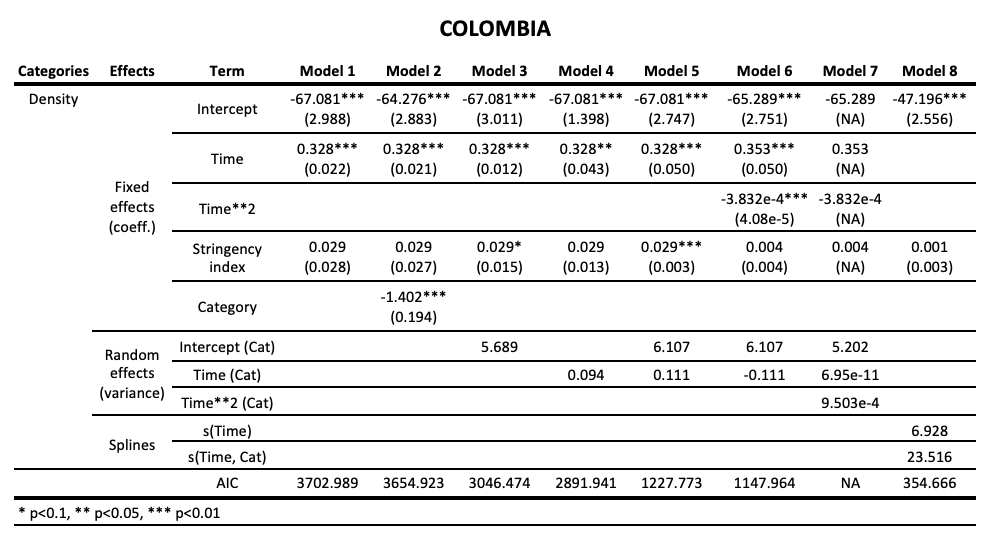
\includegraphics[width=\linewidth]{supplementary/models-tables/models-table-COL-quadratic-capital-stringency-r1.png}
\caption{Results of mixed-effects and Generalised Additive Model (GAM) models for trend analysis of relative change in netflows involving urban region surrounding capital in Colombia including stringency index as a predictor variable. Netflows are defined as inflows to an urban core minus outflows from the urban core. Random effects and spline terms according to population density.}
\label{tab-modelsCOL-capital-stringency}
\end{table}

\clearpage

\subsection{Model estimates - relative change in netflows involving all urban regions}

\begin{table}[h!]
\centering
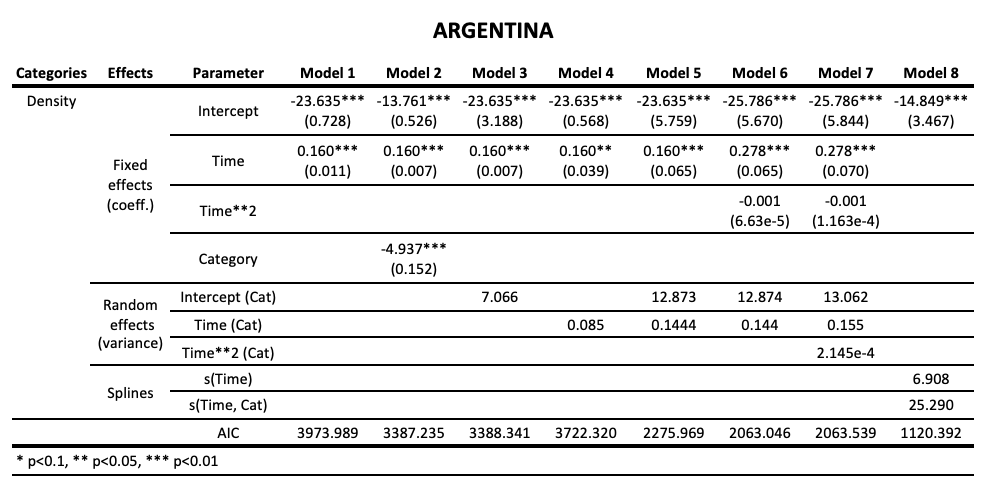
\includegraphics[width=\linewidth]{supplementary/models-tables/models-table-ARG-quadratic-fuas-r1.png}
\caption{Results of mixed-effects and Generalised Additive Model (GAM) models for trend analysis of relative change in netflows involving all urban regions in Argentina. Netflows are defined as inflows to an urban core minus outflows from the urban core. Random effects and spline terms according to population density.}
\label{tab-modelsARG-fuas}
\end{table}

\begin{table}[h!]
\centering
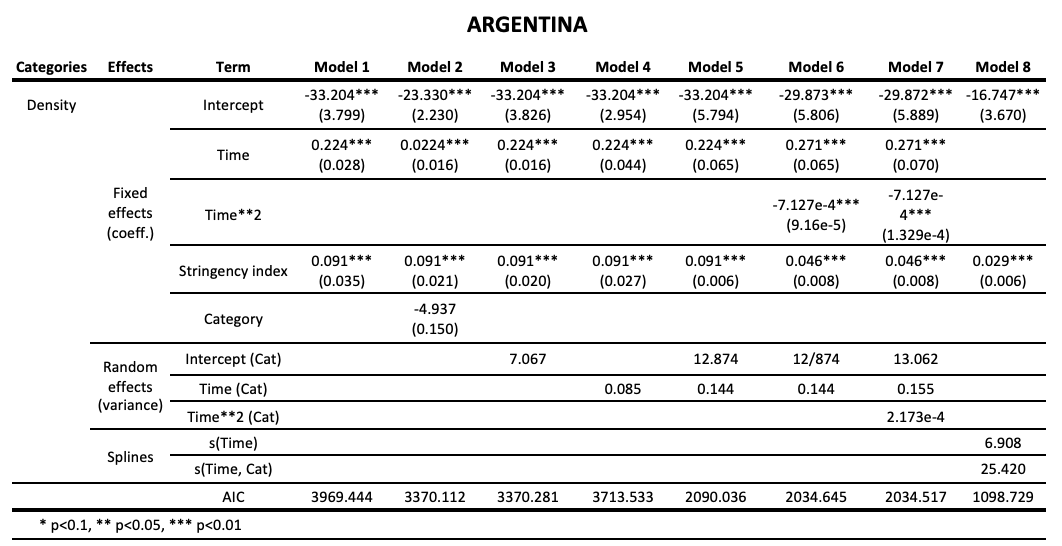
\includegraphics[width=\linewidth]{supplementary/models-tables/models-table-ARG-quadratic-fuas-stringency-r1.png}
\caption{Results of mixed-effects and Generalised Additive Model (GAM) models for trend analysis of relative change in netflows involving all urban regions in Argentina including stringency index as a predictor variable. Netflows are defined as inflows to an urban core minus outflows from the urban core. Random effects and spline terms according to population density.}
\label{tab-modelsARG-fuas-stringency}
\end{table}

\newpage

\begin{table}[h!]
\centering
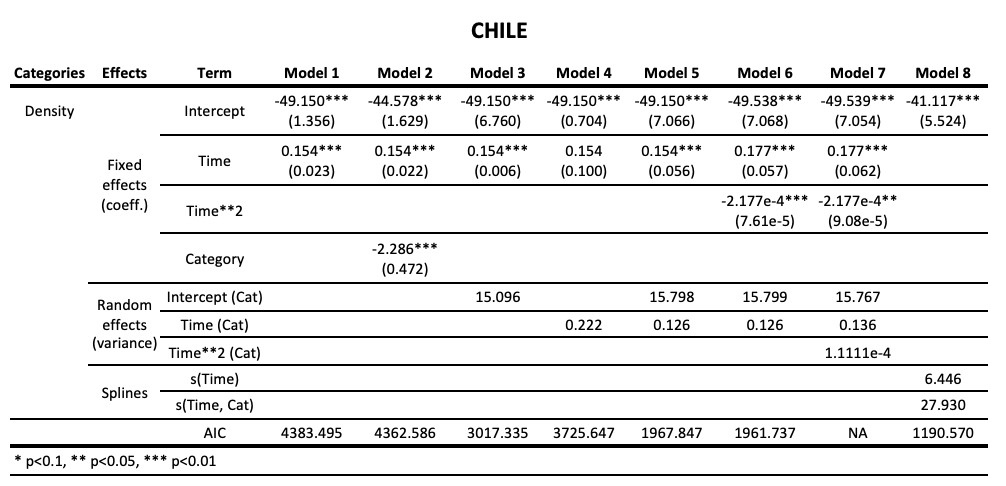
\includegraphics[width=\linewidth]{supplementary/models-tables/models-table-CHL-quadratic-fuas-r1.png}
\caption{Results of mixed-effects and Generalised Additive Model (GAM) models for trend analysis of relative change in netflows involving all urban regions in Chile. Netflows are defined as inflows to an urban core minus outflows from the urban core. Random effects and spline terms according to population density.}
\label{tab-modelsCHL-fuas}
\end{table}

\begin{table}[h!]
\centering
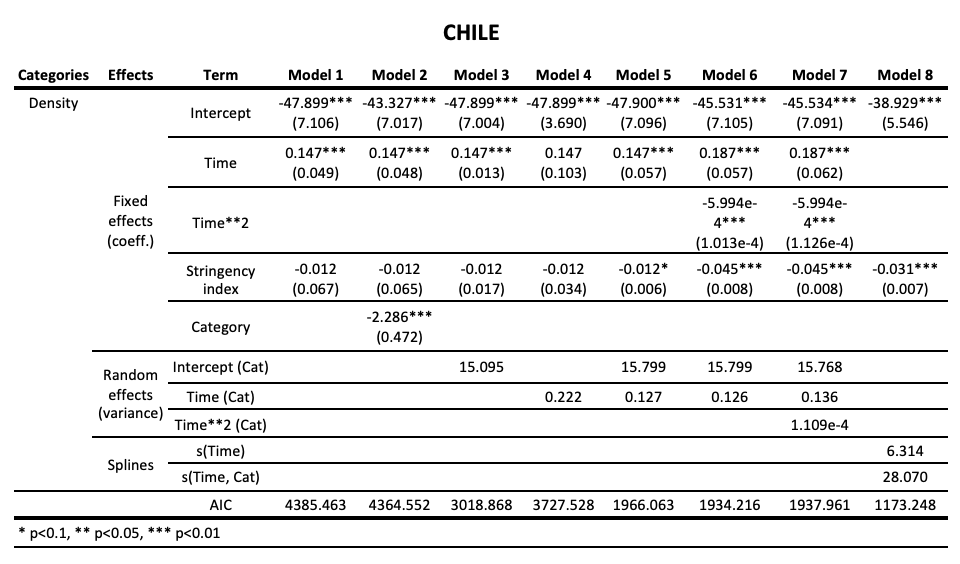
\includegraphics[width=\linewidth]{supplementary/models-tables/models-table-CHL-quadratic-fuas-stringency-r1.png}
\caption{Results of mixed-effects and Generalised Additive Model (GAM) models for trend analysis of relative change in netflows involving all urban regions in Chile including stringency index as a predictor variable. Netflows are defined as inflows to an urban core minus outflows from the urban core. Random effects and spline terms according to population density.}
\label{tab-modelsCHL-fuas-stringency}
\end{table}

\newpage

\begin{table}[h!]
\centering
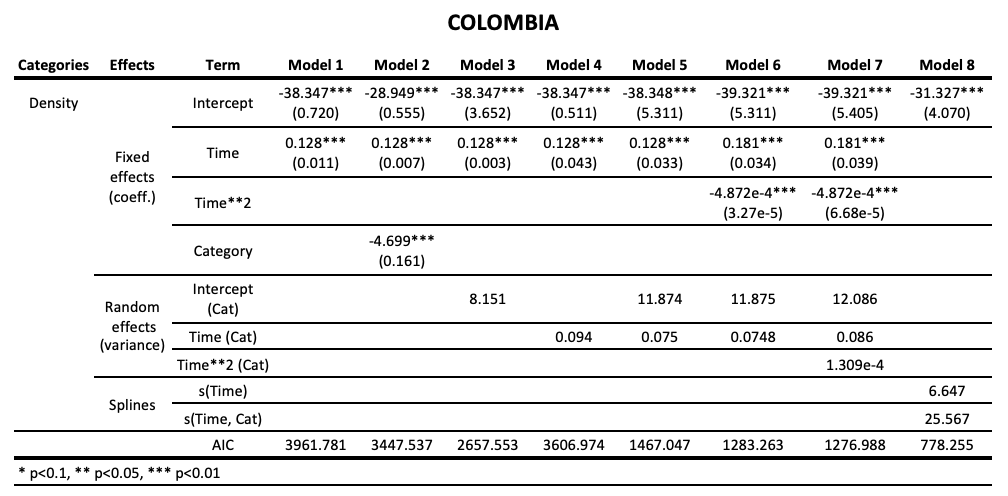
\includegraphics[width=\linewidth]{supplementary/models-tables/models-table-COL-quadratic-fuas-r1.png}
\caption{Results of mixed-effects and Generalised Additive Model (GAM) models for trend analysis of relative change in netflows involving all urban regions in Colombia. Netflows are defined as inflows to an urban core minus outflows from the urban core. Random effects and spline terms according to population density.}
\label{tab-modelsCOL-fuas}
\end{table}

\begin{table}[h!]
\centering
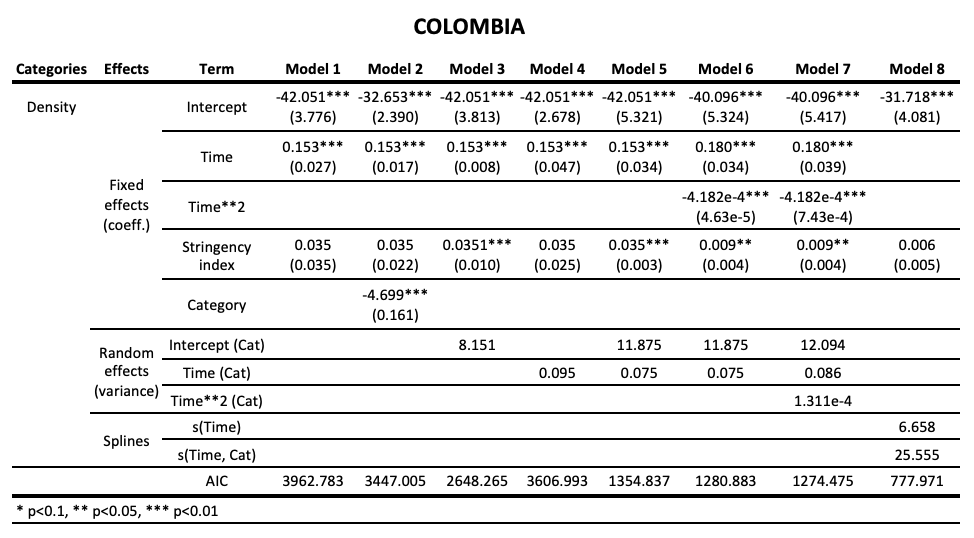
\includegraphics[width=\linewidth]{supplementary/models-tables/models-table-COL-quadratic-fuas-stringency-r1.png}
\caption{Results of mixed-effects and Generalised Additive Model (GAM) models for trend analysis of relative change in netflows involving all urban regions in Colombia including stringency index as a predictor variable. Netflows are defined as inflows to an urban core minus outflows from the urban core. Random effects and spline terms according to population density.}
\label{tab-modelsCOL-fuas-stringency}
\end{table}

\newpage

\section{Recovery times}

\subsection{Deriving recovery time formula (equation 7)}

We begin by assuming a quadratic model to describe the evolution of mobility levels over time relative to the baseline:
\begin{equation}
    y(t) = a + b\cdot t + c\cdot t^2
\end{equation}\label{model-trend}

The coefficients \( a \), \( b \), and \( c \) can be expressed in terms of the parameters from equation (6) in the main text. For instance, under Model 6, we have \( a = \beta_0 + b_0 \), \( b = \beta_1 + b_{1i} \), and \( c = \beta_2 \).

The recovery time to a threshold \( \alpha \), denoted by \( t_{\alpha} \), is defined as the time it takes for \( y(t) \) to recover by \( \alpha\% \). If the mobility level relative to the baseline at time \( t = 0 \) is \( a \), then \( t_{\alpha} \) is the time at which
\[
y(t_{\alpha}) = \left(1 - \frac{\alpha}{100}\right) a.
\]

Substituting this into equation \eqref{model-trend} and solving for \( t_{\alpha} \), we obtain:
\begin{equation}
    t_{\alpha} = \frac{-b \pm \sqrt{b^2 - 4c \left( \frac{\alpha}{100} \right) a}}{2c}
\end{equation}\label{recovery-time}

A recovery time is only meaningful if mobility initially decreased relative to the baseline, which imposes the condition \( a < 0 \). Moreover, since we are referring to a ``recovery,'' the trend must be increasing at \( t = 0 \), requiring \( y'(0) > 0 \), or equivalently, \( b > 0 \). As we are only interested in positive time values, and given \( b > 0 \), we select the solution with the \( + \) sign in equation \eqref{recovery-time}.

Finally, if \( b^2 - 4c \left( \frac{\alpha}{100} \right) a < 0 \), there is no real-valued solution for \( t_{\alpha} \). In such cases, we interpret this as mobility levels never reaching the specified recovery threshold.

The recovery time can also be obtained under a linear model (e.g. Model 5). The derivation is then analogous, but $y(t) = a + b\cdot t$ and therefore, $t_\alpha$ is given by:
\begin{equation}
    t_{\alpha} = -\dfrac{\alpha}{100}\cdot \dfrac{a}{b}
\end{equation}

\subsection{Computation of uncertainty for recovery times}

According to Model 6, the recovery time at threshold $\alpha$ is given by equation \eqref{recovery-time} where $a$, $b$ and $c$ are the coefficients for the intercept, linear and quadratic terms in equation \eqref{model-trend}.

The partial derivatives are:
\[
\frac{\partial t_\alpha}{\partial a} = \frac{-\frac{\alpha}{100}}{\sqrt{b^2 - 4c\frac{\alpha}{100} a}}, \quad
\frac{\partial t_\alpha}{\partial b} = \frac{1}{2c} \left( -1 + \frac{b}{\sqrt{b^2 - 4c\frac{\alpha}{100} a}} \right), \quad
\frac{\partial t_\alpha}{\partial c} = \frac{(b - \sqrt{b^2 - 4c\frac{\alpha}{100} a})\sqrt{b^2 - 4c\frac{\alpha}{100} a} - 2\frac{\alpha}{100} a c}{2c^2\sqrt{b^2 - 4c\frac{\alpha}{100} a}}
\]

The propagated uncertainty is:
\[
\sigma_t = \sqrt{
\left( \frac{\partial t_\alpha}{\partial a} \right)^2 \sigma_a^2 +
\left( \frac{\partial t_\alpha}{\partial b} \right)^2 \sigma_b^2 +
\left( \frac{\partial t_\alpha}{\partial c} \right)^2 \sigma_c^2}
\]

If using a linear model to estimate $t_{\alpha}$, like Model 5, then:
\[
\frac{\partial t_\alpha}{\partial a} = -\frac{\alpha}{100} \cdot \frac{1}{b}, \quad
\frac{\partial t_\alpha}{\partial b} = \dfrac{\alpha}{100}\cdot\dfrac{a}{b^2}
\]
and the propagated uncertainty is 
\begin{displaymath}
    \sigma_{t_\alpha} = \sqrt{
\left( \frac{\partial t_\alpha}{\partial a} \right)^2 \sigma_a^2 +
\left( \frac{\partial t_\alpha}{\partial b} \right)^2 \sigma_b^2 }
\end{displaymath}

\newpage

\subsection{Estimated recovery times}

\begin{table}[h!]
\centering
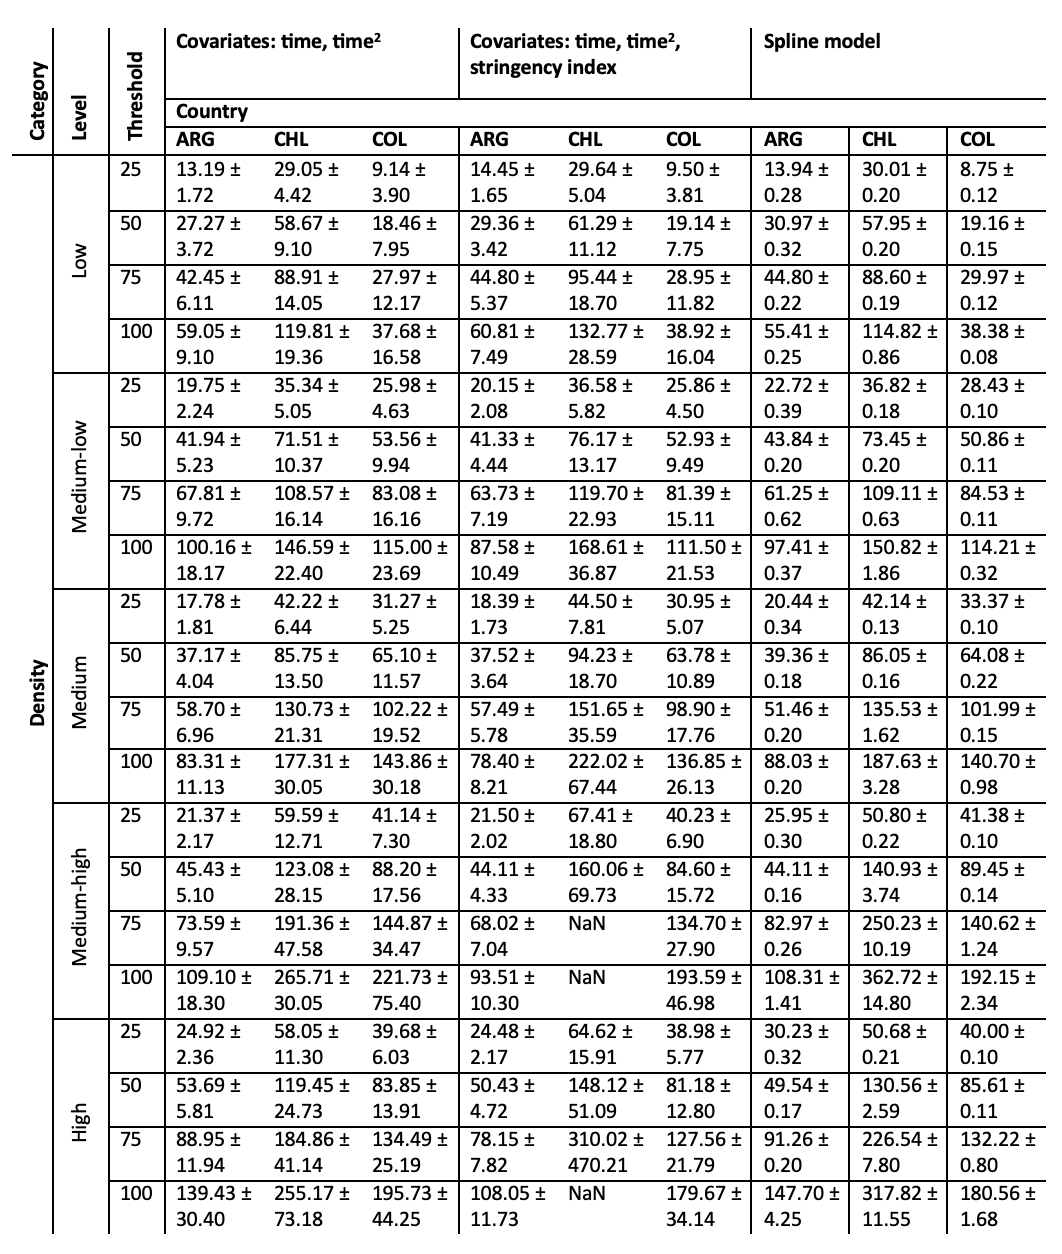
\includegraphics[width=0.9\linewidth]{supplementary/recovery-times/recovery-thresholds-table-quadratic-std-density-r1.png}
\caption{Recovery times at multiple thresholds, for outflows in Argentina, Chile and Colombia, by population density. Computed using Model 6 (with covariates time and time$^2$, or time, time$^2$ and stringency index) or according to the GAM model (Model 8). N/A values correspond to cases where the initial mobility levels are above the baseline. NaN values correspond to cases where mobility never recovers to the specified threshold.}
\end{table}

\begin{table}[h!]
\centering
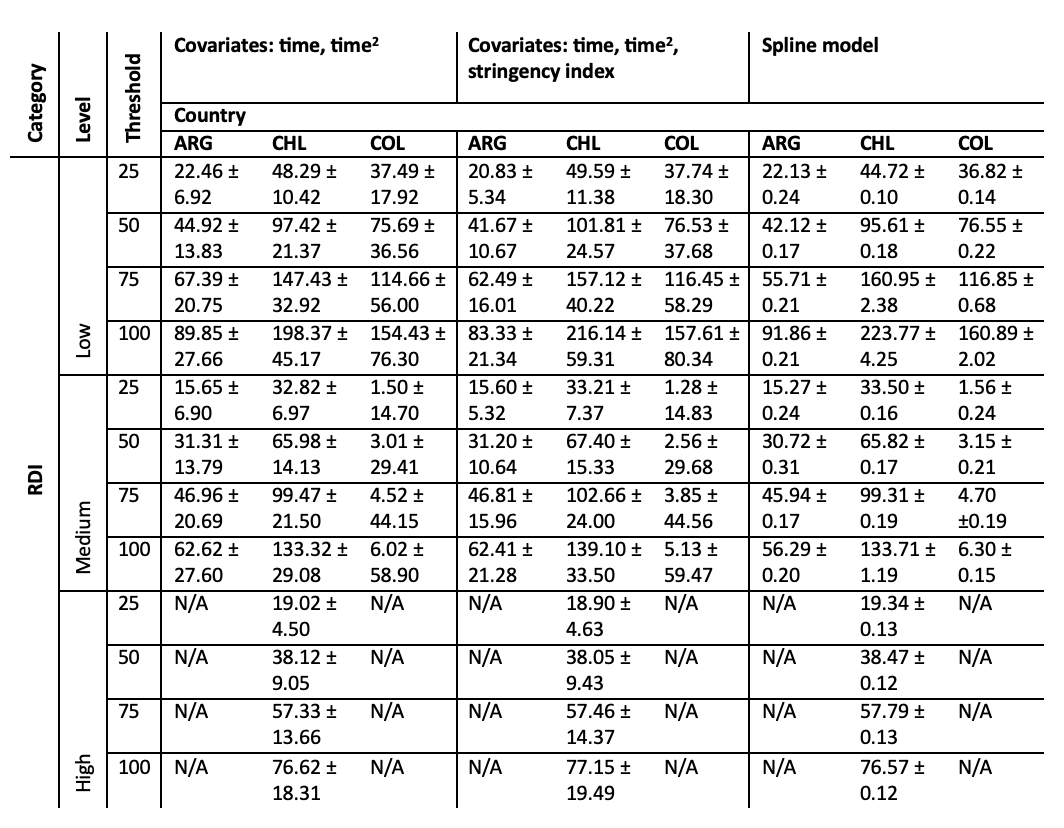
\includegraphics[width=0.9\linewidth]{supplementary/recovery-times/recovery-thresholds-table-quadratic-std-rdi-r1.png}
\caption{Recovery times at multiple thresholds, for outflows in Argentina, Chile and Colombia, by Relative Deprivation Index (RDI) category. Computed using Model 6 (with covariates time and time$^2$, or time, time$^2$ and stringency index) or according to the GAM model (Model 8). N/A values correspond to cases where the initial mobility levels are above the baseline. NaN values correspond to cases where mobility never recovers to the specified threshold.}
\end{table}

\begin{table}[h!]
\centering
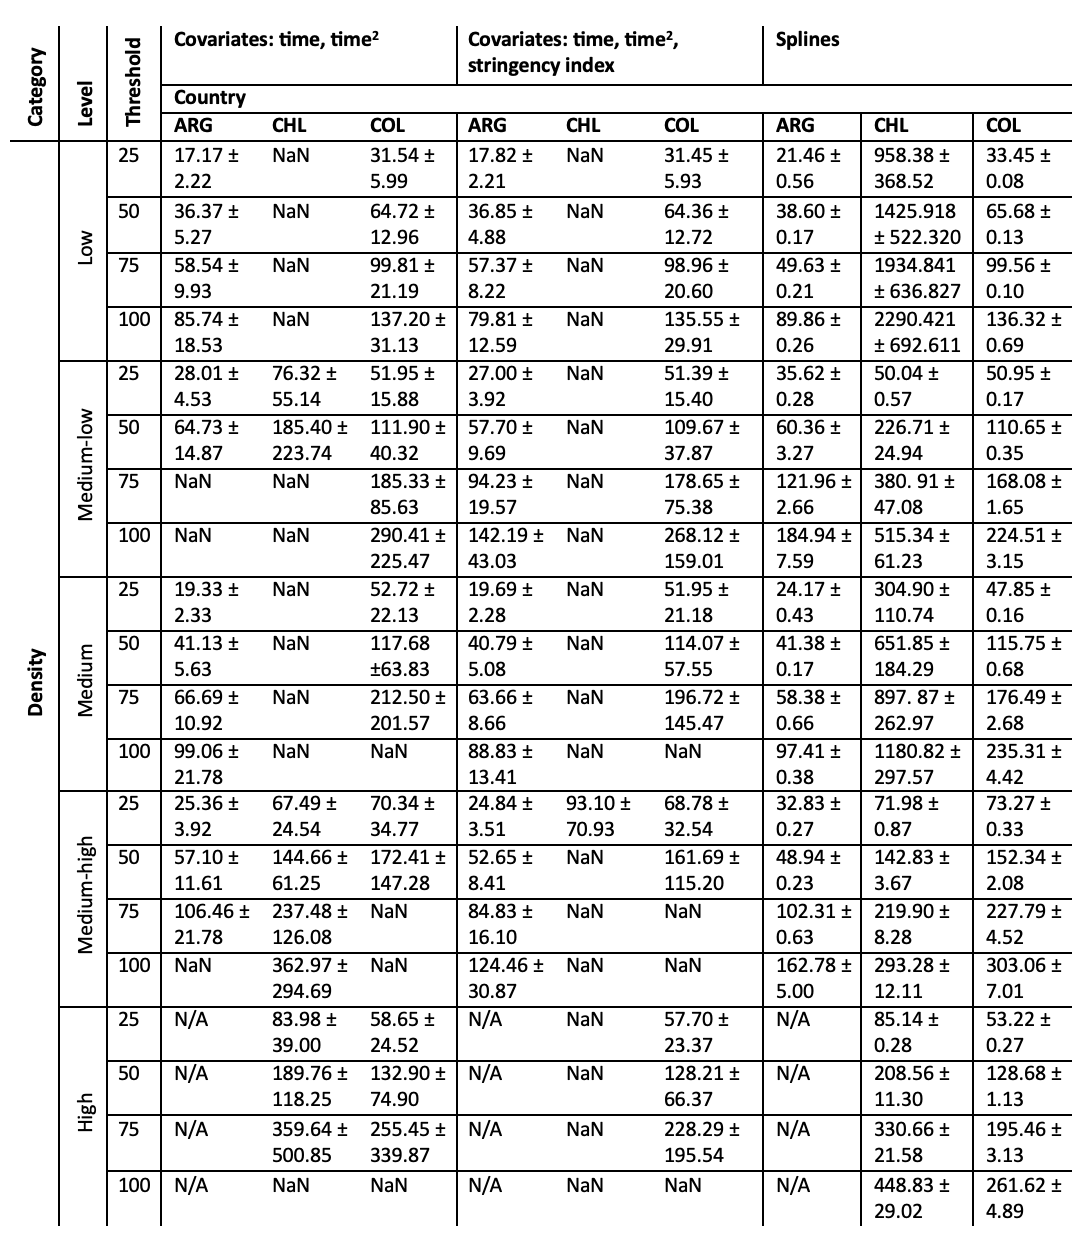
\includegraphics[width=0.9\linewidth]{supplementary/recovery-times/recovery-thresholds-table-quadratic-capital-std-r1.png}
\caption{Recovery times at multiple thresholds, for netflows involving the urban region surrounding the capital in Argentina, Chile and Colombia, by population density category. Computed using Model 6 (with covariates time and time$^2$, or time, time$^2$ and stringency index) or according to the GAM model (Model 8). N/A values correspond to cases where the initial mobility levels are above the baseline or the only cell in a population density category is the centre of netflows. NaN values correspond to cases where mobility never recovers to the specified threshold.}
\label{tab-rec-times-capital}
\end{table}

\begin{table}[h!]
\centering
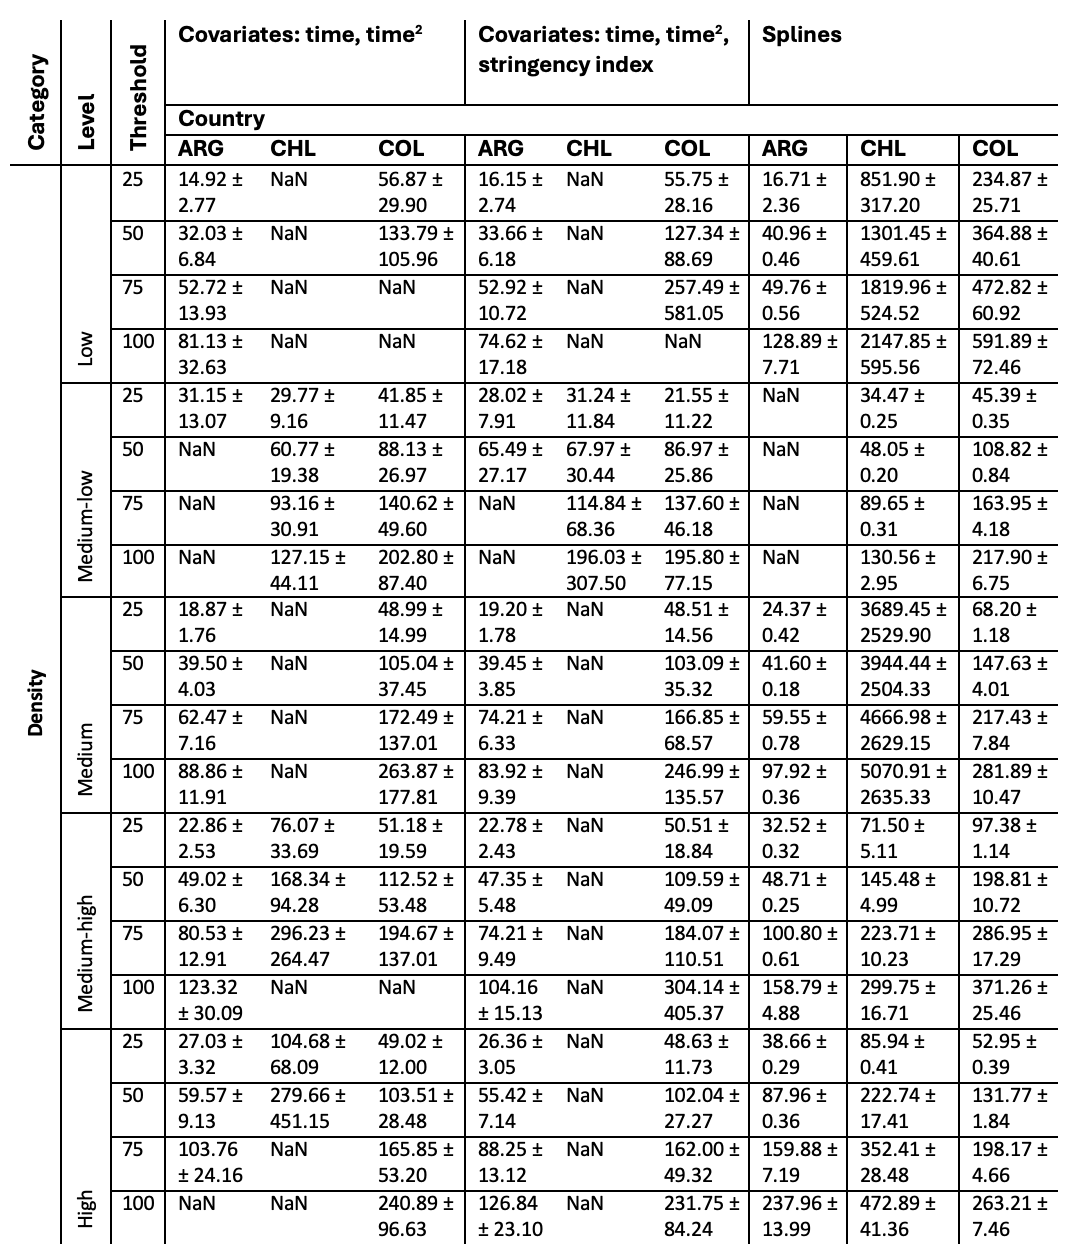
\includegraphics[width=0.9\linewidth]{supplementary/recovery-times/recovery-thresholds-table-quadratic-fuas-std-r1.png}
\caption{Recovery times at multiple thresholds, for netflows involving all urban regions in Argentina, Chile and Colombia, by population density category. Computed using Model 6 (with covariates time and time$^2$, or time, time$^2$ and stringency index) or according to the GAM model (Model 8). NaN values correspond to cases where mobility never recovers to the specified threshold.}
\label{tab-rec-times-fuas}
\end{table}

\end{document}